% Created by tikzDevice version 0.12 on 2018-10-10 11:34:15
% !TEX encoding = UTF-8 Unicode
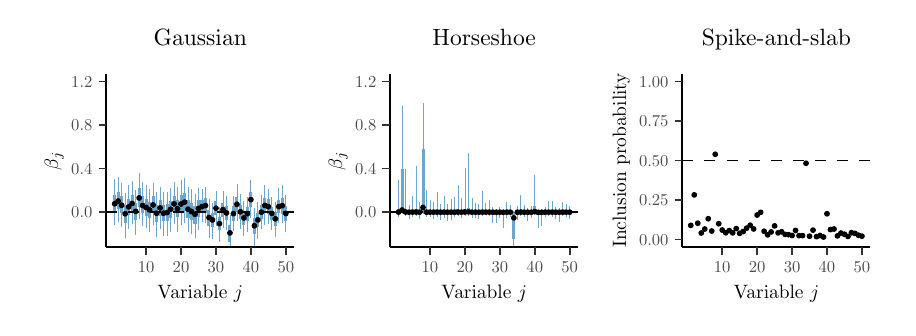
\begin{tikzpicture}[x=1pt,y=1pt]
\definecolor{fillColor}{RGB}{255,255,255}
\path[use as bounding box,fill=fillColor,fill opacity=0.00] (0,0) rectangle (310.76,101.18);
\begin{scope}
\path[clip] (  0.00, 85.87) rectangle (102.59,101.18);
\definecolor{drawColor}{RGB}{255,255,255}
\definecolor{fillColor}{RGB}{255,255,255}

\path[draw=drawColor,line width= 0.6pt,line join=round,line cap=round,fill=fillColor] ( -0.00, 85.87) rectangle (102.59,101.18);
\end{scope}
\begin{scope}
\path[clip] (  0.00,  0.00) rectangle (102.59, 85.87);
\definecolor{drawColor}{RGB}{255,255,255}
\definecolor{fillColor}{RGB}{255,255,255}

\path[draw=drawColor,line width= 0.6pt,line join=round,line cap=round,fill=fillColor] ( -0.00, -0.00) rectangle (102.59, 85.87);
\end{scope}
\begin{scope}
\path[clip] (102.59, 85.87) rectangle (205.17,101.18);
\definecolor{drawColor}{RGB}{255,255,255}
\definecolor{fillColor}{RGB}{255,255,255}

\path[draw=drawColor,line width= 0.6pt,line join=round,line cap=round,fill=fillColor] (102.59, 85.87) rectangle (205.17,101.18);
\end{scope}
\begin{scope}
\path[clip] (102.59,  0.00) rectangle (205.17, 85.87);
\definecolor{drawColor}{RGB}{255,255,255}
\definecolor{fillColor}{RGB}{255,255,255}

\path[draw=drawColor,line width= 0.6pt,line join=round,line cap=round,fill=fillColor] (102.59, -0.00) rectangle (205.17, 85.87);
\end{scope}
\begin{scope}
\path[clip] (205.17, 85.87) rectangle (310.76,101.18);
\definecolor{drawColor}{RGB}{255,255,255}
\definecolor{fillColor}{RGB}{255,255,255}

\path[draw=drawColor,line width= 0.6pt,line join=round,line cap=round,fill=fillColor] (205.17, 85.87) rectangle (310.76,101.18);
\end{scope}
\begin{scope}
\path[clip] (205.17,  0.00) rectangle (310.76, 85.87);
\definecolor{drawColor}{RGB}{255,255,255}
\definecolor{fillColor}{RGB}{255,255,255}

\path[draw=drawColor,line width= 0.6pt,line join=round,line cap=round,fill=fillColor] (205.17, -0.00) rectangle (310.76, 85.87);
\end{scope}
\begin{scope}
\path[clip] ( 28.35, 88.62) rectangle ( 96.37,101.18);
\definecolor{drawColor}{RGB}{0,0,0}

\node[text=drawColor,anchor=base,inner sep=0pt, outer sep=0pt, scale=  0.85] at ( 62.36, 94.73) {Gaussian};
\end{scope}
\begin{scope}
\path[clip] ( 28.35, 21.81) rectangle ( 96.37, 84.60);
\definecolor{fillColor}{RGB}{255,255,255}

\path[fill=fillColor] ( 28.35, 21.81) rectangle ( 96.37, 84.60);
\definecolor{drawColor}{RGB}{108,166,205}

\path[draw=drawColor,line width= 1.1pt,line join=round] ( 31.44, 40.87) --
	( 31.44, 40.87);

\path[draw=drawColor,line width= 1.1pt,line join=round] ( 31.44, 40.87) --
	( 31.44, 34.56);

\path[draw=drawColor,line width= 1.1pt,line join=round] ( 31.44, 34.56) --
	( 31.44, 34.56);

\path[draw=drawColor,line width= 1.1pt,line join=round] ( 32.70, 41.81) --
	( 32.70, 41.81);

\path[draw=drawColor,line width= 1.1pt,line join=round] ( 32.70, 41.81) --
	( 32.70, 35.51);

\path[draw=drawColor,line width= 1.1pt,line join=round] ( 32.70, 35.51) --
	( 32.70, 35.51);

\path[draw=drawColor,line width= 1.1pt,line join=round] ( 33.96, 40.18) --
	( 33.96, 40.18);

\path[draw=drawColor,line width= 1.1pt,line join=round] ( 33.96, 40.18) --
	( 33.96, 34.06);

\path[draw=drawColor,line width= 1.1pt,line join=round] ( 33.96, 34.06) --
	( 33.96, 34.06);

\path[draw=drawColor,line width= 1.1pt,line join=round] ( 35.22, 36.94) --
	( 35.22, 36.94);

\path[draw=drawColor,line width= 1.1pt,line join=round] ( 35.22, 36.94) --
	( 35.22, 30.65);

\path[draw=drawColor,line width= 1.1pt,line join=round] ( 35.22, 30.65) --
	( 35.22, 30.65);

\path[draw=drawColor,line width= 1.1pt,line join=round] ( 36.49, 39.44) --
	( 36.49, 39.44);

\path[draw=drawColor,line width= 1.1pt,line join=round] ( 36.49, 39.44) --
	( 36.49, 33.31);

\path[draw=drawColor,line width= 1.1pt,line join=round] ( 36.49, 33.31) --
	( 36.49, 33.31);

\path[draw=drawColor,line width= 1.1pt,line join=round] ( 37.75, 40.87) --
	( 37.75, 40.87);

\path[draw=drawColor,line width= 1.1pt,line join=round] ( 37.75, 40.87) --
	( 37.75, 34.64);

\path[draw=drawColor,line width= 1.1pt,line join=round] ( 37.75, 34.64) --
	( 37.75, 34.64);

\path[draw=drawColor,line width= 1.1pt,line join=round] ( 39.01, 37.68) --
	( 39.01, 37.68);

\path[draw=drawColor,line width= 1.1pt,line join=round] ( 39.01, 37.68) --
	( 39.01, 31.76);

\path[draw=drawColor,line width= 1.1pt,line join=round] ( 39.01, 31.76) --
	( 39.01, 31.76);

\path[draw=drawColor,line width= 1.1pt,line join=round] ( 40.27, 43.13) --
	( 40.27, 43.13);

\path[draw=drawColor,line width= 1.1pt,line join=round] ( 40.27, 43.13) --
	( 40.27, 36.46);

\path[draw=drawColor,line width= 1.1pt,line join=round] ( 40.27, 36.46) --
	( 40.27, 36.46);

\path[draw=drawColor,line width= 1.1pt,line join=round] ( 41.53, 40.18) --
	( 41.53, 40.18);

\path[draw=drawColor,line width= 1.1pt,line join=round] ( 41.53, 40.18) --
	( 41.53, 34.04);

\path[draw=drawColor,line width= 1.1pt,line join=round] ( 41.53, 34.04) --
	( 41.53, 34.04);

\path[draw=drawColor,line width= 1.1pt,line join=round] ( 42.80, 39.37) --
	( 42.80, 39.37);

\path[draw=drawColor,line width= 1.1pt,line join=round] ( 42.80, 39.37) --
	( 42.80, 33.22);

\path[draw=drawColor,line width= 1.1pt,line join=round] ( 42.80, 33.22) --
	( 42.80, 33.22);

\path[draw=drawColor,line width= 1.1pt,line join=round] ( 44.06, 38.29) --
	( 44.06, 38.29);

\path[draw=drawColor,line width= 1.1pt,line join=round] ( 44.06, 38.29) --
	( 44.06, 32.30);

\path[draw=drawColor,line width= 1.1pt,line join=round] ( 44.06, 32.30) --
	( 44.06, 32.30);

\path[draw=drawColor,line width= 1.1pt,line join=round] ( 45.32, 40.34) --
	( 45.32, 40.34);

\path[draw=drawColor,line width= 1.1pt,line join=round] ( 45.32, 40.34) --
	( 45.32, 34.18);

\path[draw=drawColor,line width= 1.1pt,line join=round] ( 45.32, 34.18) --
	( 45.32, 34.18);

\path[draw=drawColor,line width= 1.1pt,line join=round] ( 46.58, 37.17) --
	( 46.58, 37.17);

\path[draw=drawColor,line width= 1.1pt,line join=round] ( 46.58, 37.17) --
	( 46.58, 30.86);

\path[draw=drawColor,line width= 1.1pt,line join=round] ( 46.58, 30.86) --
	( 46.58, 30.86);

\path[draw=drawColor,line width= 1.1pt,line join=round] ( 47.84, 39.07) --
	( 47.84, 39.07);

\path[draw=drawColor,line width= 1.1pt,line join=round] ( 47.84, 39.07) --
	( 47.84, 32.98);

\path[draw=drawColor,line width= 1.1pt,line join=round] ( 47.84, 32.98) --
	( 47.84, 32.98);

\path[draw=drawColor,line width= 1.1pt,line join=round] ( 49.11, 37.21) --
	( 49.11, 37.21);

\path[draw=drawColor,line width= 1.1pt,line join=round] ( 49.11, 37.21) --
	( 49.11, 31.19);

\path[draw=drawColor,line width= 1.1pt,line join=round] ( 49.11, 31.19) --
	( 49.11, 31.19);

\path[draw=drawColor,line width= 1.1pt,line join=round] ( 50.37, 37.33) --
	( 50.37, 37.33);

\path[draw=drawColor,line width= 1.1pt,line join=round] ( 50.37, 37.33) --
	( 50.37, 31.32);

\path[draw=drawColor,line width= 1.1pt,line join=round] ( 50.37, 31.32) --
	( 50.37, 31.32);

\path[draw=drawColor,line width= 1.1pt,line join=round] ( 51.63, 38.58) --
	( 51.63, 38.58);

\path[draw=drawColor,line width= 1.1pt,line join=round] ( 51.63, 38.58) --
	( 51.63, 32.40);

\path[draw=drawColor,line width= 1.1pt,line join=round] ( 51.63, 32.40) --
	( 51.63, 32.40);

\path[draw=drawColor,line width= 1.1pt,line join=round] ( 52.89, 40.48) --
	( 52.89, 40.48);

\path[draw=drawColor,line width= 1.1pt,line join=round] ( 52.89, 40.48) --
	( 52.89, 34.62);

\path[draw=drawColor,line width= 1.1pt,line join=round] ( 52.89, 34.62) --
	( 52.89, 34.62);

\path[draw=drawColor,line width= 1.1pt,line join=round] ( 54.15, 38.90) --
	( 54.15, 38.90);

\path[draw=drawColor,line width= 1.1pt,line join=round] ( 54.15, 38.90) --
	( 54.15, 32.70);

\path[draw=drawColor,line width= 1.1pt,line join=round] ( 54.15, 32.70) --
	( 54.15, 32.70);

\path[draw=drawColor,line width= 1.1pt,line join=round] ( 55.42, 40.73) --
	( 55.42, 40.73);

\path[draw=drawColor,line width= 1.1pt,line join=round] ( 55.42, 40.73) --
	( 55.42, 34.41);

\path[draw=drawColor,line width= 1.1pt,line join=round] ( 55.42, 34.41) --
	( 55.42, 34.41);

\path[draw=drawColor,line width= 1.1pt,line join=round] ( 56.68, 41.31) --
	( 56.68, 41.31);

\path[draw=drawColor,line width= 1.1pt,line join=round] ( 56.68, 41.31) --
	( 56.68, 35.04);

\path[draw=drawColor,line width= 1.1pt,line join=round] ( 56.68, 35.04) --
	( 56.68, 35.04);

\path[draw=drawColor,line width= 1.1pt,line join=round] ( 57.94, 38.75) --
	( 57.94, 38.75);

\path[draw=drawColor,line width= 1.1pt,line join=round] ( 57.94, 38.75) --
	( 57.94, 32.33);

\path[draw=drawColor,line width= 1.1pt,line join=round] ( 57.94, 32.33) --
	( 57.94, 32.33);

\path[draw=drawColor,line width= 1.1pt,line join=round] ( 59.20, 37.84) --
	( 59.20, 37.84);

\path[draw=drawColor,line width= 1.1pt,line join=round] ( 59.20, 37.84) --
	( 59.20, 31.53);

\path[draw=drawColor,line width= 1.1pt,line join=round] ( 59.20, 31.53) --
	( 59.20, 31.53);

\path[draw=drawColor,line width= 1.1pt,line join=round] ( 60.47, 36.75) --
	( 60.47, 36.75);

\path[draw=drawColor,line width= 1.1pt,line join=round] ( 60.47, 36.75) --
	( 60.47, 30.37);

\path[draw=drawColor,line width= 1.1pt,line join=round] ( 60.47, 30.37) --
	( 60.47, 30.37);

\path[draw=drawColor,line width= 1.1pt,line join=round] ( 61.73, 38.75) --
	( 61.73, 38.75);

\path[draw=drawColor,line width= 1.1pt,line join=round] ( 61.73, 38.75) --
	( 61.73, 32.87);

\path[draw=drawColor,line width= 1.1pt,line join=round] ( 61.73, 32.87) --
	( 61.73, 32.87);

\path[draw=drawColor,line width= 1.1pt,line join=round] ( 62.99, 39.08) --
	( 62.99, 39.08);

\path[draw=drawColor,line width= 1.1pt,line join=round] ( 62.99, 39.08) --
	( 62.99, 34.19);

\path[draw=drawColor,line width= 1.1pt,line join=round] ( 62.99, 34.19) --
	( 62.99, 34.19);

\path[draw=drawColor,line width= 1.1pt,line join=round] ( 64.25, 39.46) --
	( 64.25, 39.46);

\path[draw=drawColor,line width= 1.1pt,line join=round] ( 64.25, 39.46) --
	( 64.25, 34.39);

\path[draw=drawColor,line width= 1.1pt,line join=round] ( 64.25, 34.39) --
	( 64.25, 34.39);

\path[draw=drawColor,line width= 1.1pt,line join=round] ( 65.51, 35.40) --
	( 65.51, 35.40);

\path[draw=drawColor,line width= 1.1pt,line join=round] ( 65.51, 35.40) --
	( 65.51, 29.66);

\path[draw=drawColor,line width= 1.1pt,line join=round] ( 65.51, 29.66) --
	( 65.51, 29.66);

\path[draw=drawColor,line width= 1.1pt,line join=round] ( 66.78, 34.24) --
	( 66.78, 34.24);

\path[draw=drawColor,line width= 1.1pt,line join=round] ( 66.78, 34.24) --
	( 66.78, 29.03);

\path[draw=drawColor,line width= 1.1pt,line join=round] ( 66.78, 29.03) --
	( 66.78, 29.03);

\path[draw=drawColor,line width= 1.1pt,line join=round] ( 68.04, 38.41) --
	( 68.04, 38.41);

\path[draw=drawColor,line width= 1.1pt,line join=round] ( 68.04, 38.41) --
	( 68.04, 33.42);

\path[draw=drawColor,line width= 1.1pt,line join=round] ( 68.04, 33.42) --
	( 68.04, 33.42);

\path[draw=drawColor,line width= 1.1pt,line join=round] ( 69.30, 32.82) --
	( 69.30, 32.82);

\path[draw=drawColor,line width= 1.1pt,line join=round] ( 69.30, 32.82) --
	( 69.30, 27.95);

\path[draw=drawColor,line width= 1.1pt,line join=round] ( 69.30, 27.95) --
	( 69.30, 27.95);

\path[draw=drawColor,line width= 1.1pt,line join=round] ( 70.56, 37.98) --
	( 70.56, 37.98);

\path[draw=drawColor,line width= 1.1pt,line join=round] ( 70.56, 37.98) --
	( 70.56, 32.75);

\path[draw=drawColor,line width= 1.1pt,line join=round] ( 70.56, 32.75) --
	( 70.56, 32.75);

\path[draw=drawColor,line width= 1.1pt,line join=round] ( 71.82, 36.64) --
	( 71.82, 36.64);

\path[draw=drawColor,line width= 1.1pt,line join=round] ( 71.82, 36.64) --
	( 71.82, 31.70);

\path[draw=drawColor,line width= 1.1pt,line join=round] ( 71.82, 31.70) --
	( 71.82, 31.70);

\path[draw=drawColor,line width= 1.1pt,line join=round] ( 73.09, 29.93) --
	( 73.09, 29.93);

\path[draw=drawColor,line width= 1.1pt,line join=round] ( 73.09, 29.93) --
	( 73.09, 23.91);

\path[draw=drawColor,line width= 1.1pt,line join=round] ( 73.09, 23.91) --
	( 73.09, 23.91);

\path[draw=drawColor,line width= 1.1pt,line join=round] ( 74.35, 36.58) --
	( 74.35, 36.58);

\path[draw=drawColor,line width= 1.1pt,line join=round] ( 74.35, 36.58) --
	( 74.35, 31.35);

\path[draw=drawColor,line width= 1.1pt,line join=round] ( 74.35, 31.35) --
	( 74.35, 31.35);

\path[draw=drawColor,line width= 1.1pt,line join=round] ( 75.61, 40.12) --
	( 75.61, 40.12);

\path[draw=drawColor,line width= 1.1pt,line join=round] ( 75.61, 40.12) --
	( 75.61, 34.75);

\path[draw=drawColor,line width= 1.1pt,line join=round] ( 75.61, 34.75) --
	( 75.61, 34.75);

\path[draw=drawColor,line width= 1.1pt,line join=round] ( 76.87, 37.06) --
	( 76.87, 37.06);

\path[draw=drawColor,line width= 1.1pt,line join=round] ( 76.87, 37.06) --
	( 76.87, 32.17);

\path[draw=drawColor,line width= 1.1pt,line join=round] ( 76.87, 32.17) --
	( 76.87, 32.17);

\path[draw=drawColor,line width= 1.1pt,line join=round] ( 78.13, 34.88) --
	( 78.13, 34.88);

\path[draw=drawColor,line width= 1.1pt,line join=round] ( 78.13, 34.88) --
	( 78.13, 29.78);

\path[draw=drawColor,line width= 1.1pt,line join=round] ( 78.13, 29.78) --
	( 78.13, 29.78);

\path[draw=drawColor,line width= 1.1pt,line join=round] ( 79.40, 36.36) --
	( 79.40, 36.36);

\path[draw=drawColor,line width= 1.1pt,line join=round] ( 79.40, 36.36) --
	( 79.40, 31.47);

\path[draw=drawColor,line width= 1.1pt,line join=round] ( 79.40, 31.47) --
	( 79.40, 31.47);

\path[draw=drawColor,line width= 1.1pt,line join=round] ( 80.66, 41.82) --
	( 80.66, 41.82);

\path[draw=drawColor,line width= 1.1pt,line join=round] ( 80.66, 41.82) --
	( 80.66, 36.34);

\path[draw=drawColor,line width= 1.1pt,line join=round] ( 80.66, 36.34) --
	( 80.66, 36.34);

\path[draw=drawColor,line width= 1.1pt,line join=round] ( 81.92, 32.48) --
	( 81.92, 32.48);

\path[draw=drawColor,line width= 1.1pt,line join=round] ( 81.92, 32.48) --
	( 81.92, 26.56);

\path[draw=drawColor,line width= 1.1pt,line join=round] ( 81.92, 26.56) --
	( 81.92, 26.56);

\path[draw=drawColor,line width= 1.1pt,line join=round] ( 83.18, 34.37) --
	( 83.18, 34.37);

\path[draw=drawColor,line width= 1.1pt,line join=round] ( 83.18, 34.37) --
	( 83.18, 29.01);

\path[draw=drawColor,line width= 1.1pt,line join=round] ( 83.18, 29.01) --
	( 83.18, 29.01);

\path[draw=drawColor,line width= 1.1pt,line join=round] ( 84.45, 36.97) --
	( 84.45, 36.97);

\path[draw=drawColor,line width= 1.1pt,line join=round] ( 84.45, 36.97) --
	( 84.45, 32.03);

\path[draw=drawColor,line width= 1.1pt,line join=round] ( 84.45, 32.03) --
	( 84.45, 32.03);

\path[draw=drawColor,line width= 1.1pt,line join=round] ( 85.71, 39.74) --
	( 85.71, 39.74);

\path[draw=drawColor,line width= 1.1pt,line join=round] ( 85.71, 39.74) --
	( 85.71, 34.18);

\path[draw=drawColor,line width= 1.1pt,line join=round] ( 85.71, 34.18) --
	( 85.71, 34.18);

\path[draw=drawColor,line width= 1.1pt,line join=round] ( 86.97, 39.17) --
	( 86.97, 39.17);

\path[draw=drawColor,line width= 1.1pt,line join=round] ( 86.97, 39.17) --
	( 86.97, 33.98);

\path[draw=drawColor,line width= 1.1pt,line join=round] ( 86.97, 33.98) --
	( 86.97, 33.98);

\path[draw=drawColor,line width= 1.1pt,line join=round] ( 88.23, 36.52) --
	( 88.23, 36.52);

\path[draw=drawColor,line width= 1.1pt,line join=round] ( 88.23, 36.52) --
	( 88.23, 31.56);

\path[draw=drawColor,line width= 1.1pt,line join=round] ( 88.23, 31.56) --
	( 88.23, 31.56);

\path[draw=drawColor,line width= 1.1pt,line join=round] ( 89.49, 34.65) --
	( 89.49, 34.65);

\path[draw=drawColor,line width= 1.1pt,line join=round] ( 89.49, 34.65) --
	( 89.49, 29.47);

\path[draw=drawColor,line width= 1.1pt,line join=round] ( 89.49, 29.47) --
	( 89.49, 29.47);

\path[draw=drawColor,line width= 1.1pt,line join=round] ( 90.76, 39.03) --
	( 90.76, 39.03);

\path[draw=drawColor,line width= 1.1pt,line join=round] ( 90.76, 39.03) --
	( 90.76, 34.11);

\path[draw=drawColor,line width= 1.1pt,line join=round] ( 90.76, 34.11) --
	( 90.76, 34.11);

\path[draw=drawColor,line width= 1.1pt,line join=round] ( 92.02, 39.78) --
	( 92.02, 39.78);

\path[draw=drawColor,line width= 1.1pt,line join=round] ( 92.02, 39.78) --
	( 92.02, 34.01);

\path[draw=drawColor,line width= 1.1pt,line join=round] ( 92.02, 34.01) --
	( 92.02, 34.01);

\path[draw=drawColor,line width= 1.1pt,line join=round] ( 93.28, 36.73) --
	( 93.28, 36.73);

\path[draw=drawColor,line width= 1.1pt,line join=round] ( 93.28, 36.73) --
	( 93.28, 31.30);

\path[draw=drawColor,line width= 1.1pt,line join=round] ( 93.28, 31.30) --
	( 93.28, 31.30);

\path[draw=drawColor,line width= 0.3pt,line join=round] ( 31.44, 46.59) --
	( 31.44, 46.59);

\path[draw=drawColor,line width= 0.3pt,line join=round] ( 31.44, 46.59) --
	( 31.44, 29.99);

\path[draw=drawColor,line width= 0.3pt,line join=round] ( 31.44, 29.99) --
	( 31.44, 29.99);

\path[draw=drawColor,line width= 0.3pt,line join=round] ( 32.70, 47.37) --
	( 32.70, 47.37);

\path[draw=drawColor,line width= 0.3pt,line join=round] ( 32.70, 47.37) --
	( 32.70, 30.97);

\path[draw=drawColor,line width= 0.3pt,line join=round] ( 32.70, 30.97) --
	( 32.70, 30.97);

\path[draw=drawColor,line width= 0.3pt,line join=round] ( 33.96, 45.14) --
	( 33.96, 45.14);

\path[draw=drawColor,line width= 0.3pt,line join=round] ( 33.96, 45.14) --
	( 33.96, 29.33);

\path[draw=drawColor,line width= 0.3pt,line join=round] ( 33.96, 29.33) --
	( 33.96, 29.33);

\path[draw=drawColor,line width= 0.3pt,line join=round] ( 35.22, 41.58) --
	( 35.22, 41.58);

\path[draw=drawColor,line width= 0.3pt,line join=round] ( 35.22, 41.58) --
	( 35.22, 25.35);

\path[draw=drawColor,line width= 0.3pt,line join=round] ( 35.22, 25.35) --
	( 35.22, 25.35);

\path[draw=drawColor,line width= 0.3pt,line join=round] ( 36.49, 44.18) --
	( 36.49, 44.18);

\path[draw=drawColor,line width= 0.3pt,line join=round] ( 36.49, 44.18) --
	( 36.49, 28.44);

\path[draw=drawColor,line width= 0.3pt,line join=round] ( 36.49, 28.44) --
	( 36.49, 28.44);

\path[draw=drawColor,line width= 0.3pt,line join=round] ( 37.75, 45.70) --
	( 37.75, 45.70);

\path[draw=drawColor,line width= 0.3pt,line join=round] ( 37.75, 45.70) --
	( 37.75, 30.31);

\path[draw=drawColor,line width= 0.3pt,line join=round] ( 37.75, 30.31) --
	( 37.75, 30.31);

\path[draw=drawColor,line width= 0.3pt,line join=round] ( 39.01, 42.40) --
	( 39.01, 42.40);

\path[draw=drawColor,line width= 0.3pt,line join=round] ( 39.01, 42.40) --
	( 39.01, 26.43);

\path[draw=drawColor,line width= 0.3pt,line join=round] ( 39.01, 26.43) --
	( 39.01, 26.43);

\path[draw=drawColor,line width= 0.3pt,line join=round] ( 40.27, 48.75) --
	( 40.27, 48.75);

\path[draw=drawColor,line width= 0.3pt,line join=round] ( 40.27, 48.75) --
	( 40.27, 32.19);

\path[draw=drawColor,line width= 0.3pt,line join=round] ( 40.27, 32.19) --
	( 40.27, 32.19);

\path[draw=drawColor,line width= 0.3pt,line join=round] ( 41.53, 45.57) --
	( 41.53, 45.57);

\path[draw=drawColor,line width= 0.3pt,line join=round] ( 41.53, 45.57) --
	( 41.53, 29.34);

\path[draw=drawColor,line width= 0.3pt,line join=round] ( 41.53, 29.34) --
	( 41.53, 29.34);

\path[draw=drawColor,line width= 0.3pt,line join=round] ( 42.80, 44.35) --
	( 42.80, 44.35);

\path[draw=drawColor,line width= 0.3pt,line join=round] ( 42.80, 44.35) --
	( 42.80, 28.87);

\path[draw=drawColor,line width= 0.3pt,line join=round] ( 42.80, 28.87) --
	( 42.80, 28.87);

\path[draw=drawColor,line width= 0.3pt,line join=round] ( 44.06, 42.91) --
	( 44.06, 42.91);

\path[draw=drawColor,line width= 0.3pt,line join=round] ( 44.06, 42.91) --
	( 44.06, 27.19);

\path[draw=drawColor,line width= 0.3pt,line join=round] ( 44.06, 27.19) --
	( 44.06, 27.19);

\path[draw=drawColor,line width= 0.3pt,line join=round] ( 45.32, 45.17) --
	( 45.32, 45.17);

\path[draw=drawColor,line width= 0.3pt,line join=round] ( 45.32, 45.17) --
	( 45.32, 29.77);

\path[draw=drawColor,line width= 0.3pt,line join=round] ( 45.32, 29.77) --
	( 45.32, 29.77);

\path[draw=drawColor,line width= 0.3pt,line join=round] ( 46.58, 41.71) --
	( 46.58, 41.71);

\path[draw=drawColor,line width= 0.3pt,line join=round] ( 46.58, 41.71) --
	( 46.58, 25.45);

\path[draw=drawColor,line width= 0.3pt,line join=round] ( 46.58, 25.45) --
	( 46.58, 25.45);

\path[draw=drawColor,line width= 0.3pt,line join=round] ( 47.84, 43.70) --
	( 47.84, 43.70);

\path[draw=drawColor,line width= 0.3pt,line join=round] ( 47.84, 43.70) --
	( 47.84, 28.30);

\path[draw=drawColor,line width= 0.3pt,line join=round] ( 47.84, 28.30) --
	( 47.84, 28.30);

\path[draw=drawColor,line width= 0.3pt,line join=round] ( 49.11, 41.69) --
	( 49.11, 41.69);

\path[draw=drawColor,line width= 0.3pt,line join=round] ( 49.11, 41.69) --
	( 49.11, 26.06);

\path[draw=drawColor,line width= 0.3pt,line join=round] ( 49.11, 26.06) --
	( 49.11, 26.06);

\path[draw=drawColor,line width= 0.3pt,line join=round] ( 50.37, 41.74) --
	( 50.37, 41.74);

\path[draw=drawColor,line width= 0.3pt,line join=round] ( 50.37, 41.74) --
	( 50.37, 25.95);

\path[draw=drawColor,line width= 0.3pt,line join=round] ( 50.37, 25.95) --
	( 50.37, 25.95);

\path[draw=drawColor,line width= 0.3pt,line join=round] ( 51.63, 43.32) --
	( 51.63, 43.32);

\path[draw=drawColor,line width= 0.3pt,line join=round] ( 51.63, 43.32) --
	( 51.63, 27.41);

\path[draw=drawColor,line width= 0.3pt,line join=round] ( 51.63, 27.41) --
	( 51.63, 27.41);

\path[draw=drawColor,line width= 0.3pt,line join=round] ( 52.89, 45.33) --
	( 52.89, 45.33);

\path[draw=drawColor,line width= 0.3pt,line join=round] ( 52.89, 45.33) --
	( 52.89, 30.16);

\path[draw=drawColor,line width= 0.3pt,line join=round] ( 52.89, 30.16) --
	( 52.89, 30.16);

\path[draw=drawColor,line width= 0.3pt,line join=round] ( 54.15, 43.63) --
	( 54.15, 43.63);

\path[draw=drawColor,line width= 0.3pt,line join=round] ( 54.15, 43.63) --
	( 54.15, 27.47);

\path[draw=drawColor,line width= 0.3pt,line join=round] ( 54.15, 27.47) --
	( 54.15, 27.47);

\path[draw=drawColor,line width= 0.3pt,line join=round] ( 55.42, 46.08) --
	( 55.42, 46.08);

\path[draw=drawColor,line width= 0.3pt,line join=round] ( 55.42, 46.08) --
	( 55.42, 29.75);

\path[draw=drawColor,line width= 0.3pt,line join=round] ( 55.42, 29.75) --
	( 55.42, 29.75);

\path[draw=drawColor,line width= 0.3pt,line join=round] ( 56.68, 46.88) --
	( 56.68, 46.88);

\path[draw=drawColor,line width= 0.3pt,line join=round] ( 56.68, 46.88) --
	( 56.68, 30.54);

\path[draw=drawColor,line width= 0.3pt,line join=round] ( 56.68, 30.54) --
	( 56.68, 30.54);

\path[draw=drawColor,line width= 0.3pt,line join=round] ( 57.94, 43.62) --
	( 57.94, 43.62);

\path[draw=drawColor,line width= 0.3pt,line join=round] ( 57.94, 43.62) --
	( 57.94, 27.46);

\path[draw=drawColor,line width= 0.3pt,line join=round] ( 57.94, 27.46) --
	( 57.94, 27.46);

\path[draw=drawColor,line width= 0.3pt,line join=round] ( 59.20, 42.84) --
	( 59.20, 42.84);

\path[draw=drawColor,line width= 0.3pt,line join=round] ( 59.20, 42.84) --
	( 59.20, 26.50);

\path[draw=drawColor,line width= 0.3pt,line join=round] ( 59.20, 26.50) --
	( 59.20, 26.50);

\path[draw=drawColor,line width= 0.3pt,line join=round] ( 60.47, 41.16) --
	( 60.47, 41.16);

\path[draw=drawColor,line width= 0.3pt,line join=round] ( 60.47, 41.16) --
	( 60.47, 25.06);

\path[draw=drawColor,line width= 0.3pt,line join=round] ( 60.47, 25.06) --
	( 60.47, 25.06);

\path[draw=drawColor,line width= 0.3pt,line join=round] ( 61.73, 43.40) --
	( 61.73, 43.40);

\path[draw=drawColor,line width= 0.3pt,line join=round] ( 61.73, 43.40) --
	( 61.73, 28.12);

\path[draw=drawColor,line width= 0.3pt,line join=round] ( 61.73, 28.12) --
	( 61.73, 28.12);

\path[draw=drawColor,line width= 0.3pt,line join=round] ( 62.99, 42.84) --
	( 62.99, 42.84);

\path[draw=drawColor,line width= 0.3pt,line join=round] ( 62.99, 42.84) --
	( 62.99, 30.81);

\path[draw=drawColor,line width= 0.3pt,line join=round] ( 62.99, 30.81) --
	( 62.99, 30.81);

\path[draw=drawColor,line width= 0.3pt,line join=round] ( 64.25, 43.44) --
	( 64.25, 43.44);

\path[draw=drawColor,line width= 0.3pt,line join=round] ( 64.25, 43.44) --
	( 64.25, 30.72);

\path[draw=drawColor,line width= 0.3pt,line join=round] ( 64.25, 30.72) --
	( 64.25, 30.72);

\path[draw=drawColor,line width= 0.3pt,line join=round] ( 65.51, 39.36) --
	( 65.51, 39.36);

\path[draw=drawColor,line width= 0.3pt,line join=round] ( 65.51, 39.36) --
	( 65.51, 25.05);

\path[draw=drawColor,line width= 0.3pt,line join=round] ( 65.51, 25.05) --
	( 65.51, 25.05);

\path[draw=drawColor,line width= 0.3pt,line join=round] ( 66.78, 37.81) --
	( 66.78, 37.81);

\path[draw=drawColor,line width= 0.3pt,line join=round] ( 66.78, 37.81) --
	( 66.78, 24.72);

\path[draw=drawColor,line width= 0.3pt,line join=round] ( 66.78, 24.72) --
	( 66.78, 24.72);

\path[draw=drawColor,line width= 0.3pt,line join=round] ( 68.04, 42.28) --
	( 68.04, 42.28);

\path[draw=drawColor,line width= 0.3pt,line join=round] ( 68.04, 42.28) --
	( 68.04, 29.56);

\path[draw=drawColor,line width= 0.3pt,line join=round] ( 68.04, 29.56) --
	( 68.04, 29.56);

\path[draw=drawColor,line width= 0.3pt,line join=round] ( 69.30, 36.32) --
	( 69.30, 36.32);

\path[draw=drawColor,line width= 0.3pt,line join=round] ( 69.30, 36.32) --
	( 69.30, 23.85);

\path[draw=drawColor,line width= 0.3pt,line join=round] ( 69.30, 23.85) --
	( 69.30, 23.85);

\path[draw=drawColor,line width= 0.3pt,line join=round] ( 70.56, 42.11) --
	( 70.56, 42.11);

\path[draw=drawColor,line width= 0.3pt,line join=round] ( 70.56, 42.11) --
	( 70.56, 28.74);

\path[draw=drawColor,line width= 0.3pt,line join=round] ( 70.56, 28.74) --
	( 70.56, 28.74);

\path[draw=drawColor,line width= 0.3pt,line join=round] ( 71.82, 40.18) --
	( 71.82, 40.18);

\path[draw=drawColor,line width= 0.3pt,line join=round] ( 71.82, 40.18) --
	( 71.82, 27.97);

\path[draw=drawColor,line width= 0.3pt,line join=round] ( 71.82, 27.97) --
	( 71.82, 27.97);

\path[draw=drawColor,line width= 0.3pt,line join=round] ( 73.09, 33.61) --
	( 73.09, 33.61);

\path[draw=drawColor,line width= 0.3pt,line join=round] ( 73.09, 33.61) --
	( 73.09, 19.22);

\path[draw=drawColor,line width= 0.3pt,line join=round] ( 73.09, 19.22) --
	( 73.09, 19.22);

\path[draw=drawColor,line width= 0.3pt,line join=round] ( 74.35, 40.49) --
	( 74.35, 40.49);

\path[draw=drawColor,line width= 0.3pt,line join=round] ( 74.35, 40.49) --
	( 74.35, 27.69);

\path[draw=drawColor,line width= 0.3pt,line join=round] ( 74.35, 27.69) --
	( 74.35, 27.69);

\path[draw=drawColor,line width= 0.3pt,line join=round] ( 75.61, 44.65) --
	( 75.61, 44.65);

\path[draw=drawColor,line width= 0.3pt,line join=round] ( 75.61, 44.65) --
	( 75.61, 31.21);

\path[draw=drawColor,line width= 0.3pt,line join=round] ( 75.61, 31.21) --
	( 75.61, 31.21);

\path[draw=drawColor,line width= 0.3pt,line join=round] ( 76.87, 40.92) --
	( 76.87, 40.92);

\path[draw=drawColor,line width= 0.3pt,line join=round] ( 76.87, 40.92) --
	( 76.87, 28.46);

\path[draw=drawColor,line width= 0.3pt,line join=round] ( 76.87, 28.46) --
	( 76.87, 28.46);

\path[draw=drawColor,line width= 0.3pt,line join=round] ( 78.13, 38.57) --
	( 78.13, 38.57);

\path[draw=drawColor,line width= 0.3pt,line join=round] ( 78.13, 38.57) --
	( 78.13, 25.87);

\path[draw=drawColor,line width= 0.3pt,line join=round] ( 78.13, 25.87) --
	( 78.13, 25.87);

\path[draw=drawColor,line width= 0.3pt,line join=round] ( 79.40, 40.05) --
	( 79.40, 40.05);

\path[draw=drawColor,line width= 0.3pt,line join=round] ( 79.40, 40.05) --
	( 79.40, 27.50);

\path[draw=drawColor,line width= 0.3pt,line join=round] ( 79.40, 27.50) --
	( 79.40, 27.50);

\path[draw=drawColor,line width= 0.3pt,line join=round] ( 80.66, 46.13) --
	( 80.66, 46.13);

\path[draw=drawColor,line width= 0.3pt,line join=round] ( 80.66, 46.13) --
	( 80.66, 32.51);

\path[draw=drawColor,line width= 0.3pt,line join=round] ( 80.66, 32.51) --
	( 80.66, 32.51);

\path[draw=drawColor,line width= 0.3pt,line join=round] ( 81.92, 36.08) --
	( 81.92, 36.08);

\path[draw=drawColor,line width= 0.3pt,line join=round] ( 81.92, 36.08) --
	( 81.92, 21.68);

\path[draw=drawColor,line width= 0.3pt,line join=round] ( 81.92, 21.68) --
	( 81.92, 21.68);

\path[draw=drawColor,line width= 0.3pt,line join=round] ( 83.18, 38.27) --
	( 83.18, 38.27);

\path[draw=drawColor,line width= 0.3pt,line join=round] ( 83.18, 38.27) --
	( 83.18, 24.64);

\path[draw=drawColor,line width= 0.3pt,line join=round] ( 83.18, 24.64) --
	( 83.18, 24.64);

\path[draw=drawColor,line width= 0.3pt,line join=round] ( 84.45, 40.67) --
	( 84.45, 40.67);

\path[draw=drawColor,line width= 0.3pt,line join=round] ( 84.45, 40.67) --
	( 84.45, 28.29);

\path[draw=drawColor,line width= 0.3pt,line join=round] ( 84.45, 28.29) --
	( 84.45, 28.29);

\path[draw=drawColor,line width= 0.3pt,line join=round] ( 85.71, 44.35) --
	( 85.71, 44.35);

\path[draw=drawColor,line width= 0.3pt,line join=round] ( 85.71, 44.35) --
	( 85.71, 29.93);

\path[draw=drawColor,line width= 0.3pt,line join=round] ( 85.71, 29.93) --
	( 85.71, 29.93);

\path[draw=drawColor,line width= 0.3pt,line join=round] ( 86.97, 43.03) --
	( 86.97, 43.03);

\path[draw=drawColor,line width= 0.3pt,line join=round] ( 86.97, 43.03) --
	( 86.97, 30.13);

\path[draw=drawColor,line width= 0.3pt,line join=round] ( 86.97, 30.13) --
	( 86.97, 30.13);

\path[draw=drawColor,line width= 0.3pt,line join=round] ( 88.23, 40.07) --
	( 88.23, 40.07);

\path[draw=drawColor,line width= 0.3pt,line join=round] ( 88.23, 40.07) --
	( 88.23, 28.00);

\path[draw=drawColor,line width= 0.3pt,line join=round] ( 88.23, 28.00) --
	( 88.23, 28.00);

\path[draw=drawColor,line width= 0.3pt,line join=round] ( 89.49, 38.21) --
	( 89.49, 38.21);

\path[draw=drawColor,line width= 0.3pt,line join=round] ( 89.49, 38.21) --
	( 89.49, 25.67);

\path[draw=drawColor,line width= 0.3pt,line join=round] ( 89.49, 25.67) --
	( 89.49, 25.67);

\path[draw=drawColor,line width= 0.3pt,line join=round] ( 90.76, 43.14) --
	( 90.76, 43.14);

\path[draw=drawColor,line width= 0.3pt,line join=round] ( 90.76, 43.14) --
	( 90.76, 30.46);

\path[draw=drawColor,line width= 0.3pt,line join=round] ( 90.76, 30.46) --
	( 90.76, 30.46);

\path[draw=drawColor,line width= 0.3pt,line join=round] ( 92.02, 44.42) --
	( 92.02, 44.42);

\path[draw=drawColor,line width= 0.3pt,line join=round] ( 92.02, 44.42) --
	( 92.02, 30.43);

\path[draw=drawColor,line width= 0.3pt,line join=round] ( 92.02, 30.43) --
	( 92.02, 30.43);

\path[draw=drawColor,line width= 0.3pt,line join=round] ( 93.28, 40.81) --
	( 93.28, 40.81);

\path[draw=drawColor,line width= 0.3pt,line join=round] ( 93.28, 40.81) --
	( 93.28, 27.24);

\path[draw=drawColor,line width= 0.3pt,line join=round] ( 93.28, 27.24) --
	( 93.28, 27.24);
\definecolor{drawColor}{RGB}{0,0,0}
\definecolor{fillColor}{RGB}{0,0,0}

\path[draw=drawColor,line width= 0.4pt,line join=round,line cap=round,fill=fillColor] ( 31.44, 37.56) circle (  0.84);

\path[draw=drawColor,line width= 0.4pt,line join=round,line cap=round,fill=fillColor] ( 32.70, 38.53) circle (  0.84);

\path[draw=drawColor,line width= 0.4pt,line join=round,line cap=round,fill=fillColor] ( 33.96, 37.01) circle (  0.84);

\path[draw=drawColor,line width= 0.4pt,line join=round,line cap=round,fill=fillColor] ( 35.22, 33.94) circle (  0.84);

\path[draw=drawColor,line width= 0.4pt,line join=round,line cap=round,fill=fillColor] ( 36.49, 36.43) circle (  0.84);

\path[draw=drawColor,line width= 0.4pt,line join=round,line cap=round,fill=fillColor] ( 37.75, 37.63) circle (  0.84);

\path[draw=drawColor,line width= 0.4pt,line join=round,line cap=round,fill=fillColor] ( 39.01, 34.80) circle (  0.84);

\path[draw=drawColor,line width= 0.4pt,line join=round,line cap=round,fill=fillColor] ( 40.27, 39.65) circle (  0.84);

\path[draw=drawColor,line width= 0.4pt,line join=round,line cap=round,fill=fillColor] ( 41.53, 36.90) circle (  0.84);

\path[draw=drawColor,line width= 0.4pt,line join=round,line cap=round,fill=fillColor] ( 42.80, 36.20) circle (  0.84);

\path[draw=drawColor,line width= 0.4pt,line join=round,line cap=round,fill=fillColor] ( 44.06, 35.34) circle (  0.84);

\path[draw=drawColor,line width= 0.4pt,line join=round,line cap=round,fill=fillColor] ( 45.32, 37.13) circle (  0.84);

\path[draw=drawColor,line width= 0.4pt,line join=round,line cap=round,fill=fillColor] ( 46.58, 34.12) circle (  0.84);

\path[draw=drawColor,line width= 0.4pt,line join=round,line cap=round,fill=fillColor] ( 47.84, 36.04) circle (  0.84);

\path[draw=drawColor,line width= 0.4pt,line join=round,line cap=round,fill=fillColor] ( 49.11, 34.14) circle (  0.84);

\path[draw=drawColor,line width= 0.4pt,line join=round,line cap=round,fill=fillColor] ( 50.37, 34.36) circle (  0.84);

\path[draw=drawColor,line width= 0.4pt,line join=round,line cap=round,fill=fillColor] ( 51.63, 35.55) circle (  0.84);

\path[draw=drawColor,line width= 0.4pt,line join=round,line cap=round,fill=fillColor] ( 52.89, 37.50) circle (  0.84);

\path[draw=drawColor,line width= 0.4pt,line join=round,line cap=round,fill=fillColor] ( 54.15, 35.76) circle (  0.84);

\path[draw=drawColor,line width= 0.4pt,line join=round,line cap=round,fill=fillColor] ( 55.42, 37.47) circle (  0.84);

\path[draw=drawColor,line width= 0.4pt,line join=round,line cap=round,fill=fillColor] ( 56.68, 38.13) circle (  0.84);

\path[draw=drawColor,line width= 0.4pt,line join=round,line cap=round,fill=fillColor] ( 57.94, 35.58) circle (  0.84);

\path[draw=drawColor,line width= 0.4pt,line join=round,line cap=round,fill=fillColor] ( 59.20, 34.73) circle (  0.84);

\path[draw=drawColor,line width= 0.4pt,line join=round,line cap=round,fill=fillColor] ( 60.47, 33.75) circle (  0.84);

\path[draw=drawColor,line width= 0.4pt,line join=round,line cap=round,fill=fillColor] ( 61.73, 35.84) circle (  0.84);

\path[draw=drawColor,line width= 0.4pt,line join=round,line cap=round,fill=fillColor] ( 62.99, 36.51) circle (  0.84);

\path[draw=drawColor,line width= 0.4pt,line join=round,line cap=round,fill=fillColor] ( 64.25, 36.91) circle (  0.84);

\path[draw=drawColor,line width= 0.4pt,line join=round,line cap=round,fill=fillColor] ( 65.51, 32.57) circle (  0.84);

\path[draw=drawColor,line width= 0.4pt,line join=round,line cap=round,fill=fillColor] ( 66.78, 31.71) circle (  0.84);

\path[draw=drawColor,line width= 0.4pt,line join=round,line cap=round,fill=fillColor] ( 68.04, 35.94) circle (  0.84);

\path[draw=drawColor,line width= 0.4pt,line join=round,line cap=round,fill=fillColor] ( 69.30, 30.38) circle (  0.84);

\path[draw=drawColor,line width= 0.4pt,line join=round,line cap=round,fill=fillColor] ( 70.56, 35.43) circle (  0.84);

\path[draw=drawColor,line width= 0.4pt,line join=round,line cap=round,fill=fillColor] ( 71.82, 34.24) circle (  0.84);

\path[draw=drawColor,line width= 0.4pt,line join=round,line cap=round,fill=fillColor] ( 73.09, 27.02) circle (  0.84);

\path[draw=drawColor,line width= 0.4pt,line join=round,line cap=round,fill=fillColor] ( 74.35, 33.98) circle (  0.84);

\path[draw=drawColor,line width= 0.4pt,line join=round,line cap=round,fill=fillColor] ( 75.61, 37.35) circle (  0.84);

\path[draw=drawColor,line width= 0.4pt,line join=round,line cap=round,fill=fillColor] ( 76.87, 34.66) circle (  0.84);

\path[draw=drawColor,line width= 0.4pt,line join=round,line cap=round,fill=fillColor] ( 78.13, 32.41) circle (  0.84);

\path[draw=drawColor,line width= 0.4pt,line join=round,line cap=round,fill=fillColor] ( 79.40, 33.96) circle (  0.84);

\path[draw=drawColor,line width= 0.4pt,line join=round,line cap=round,fill=fillColor] ( 80.66, 39.05) circle (  0.84);

\path[draw=drawColor,line width= 0.4pt,line join=round,line cap=round,fill=fillColor] ( 81.92, 29.61) circle (  0.84);

\path[draw=drawColor,line width= 0.4pt,line join=round,line cap=round,fill=fillColor] ( 83.18, 31.70) circle (  0.84);

\path[draw=drawColor,line width= 0.4pt,line join=round,line cap=round,fill=fillColor] ( 84.45, 34.51) circle (  0.84);

\path[draw=drawColor,line width= 0.4pt,line join=round,line cap=round,fill=fillColor] ( 85.71, 36.96) circle (  0.84);

\path[draw=drawColor,line width= 0.4pt,line join=round,line cap=round,fill=fillColor] ( 86.97, 36.49) circle (  0.84);

\path[draw=drawColor,line width= 0.4pt,line join=round,line cap=round,fill=fillColor] ( 88.23, 34.05) circle (  0.84);

\path[draw=drawColor,line width= 0.4pt,line join=round,line cap=round,fill=fillColor] ( 89.49, 32.11) circle (  0.84);

\path[draw=drawColor,line width= 0.4pt,line join=round,line cap=round,fill=fillColor] ( 90.76, 36.51) circle (  0.84);

\path[draw=drawColor,line width= 0.4pt,line join=round,line cap=round,fill=fillColor] ( 92.02, 36.88) circle (  0.84);

\path[draw=drawColor,line width= 0.4pt,line join=round,line cap=round,fill=fillColor] ( 93.28, 34.01) circle (  0.84);

\path[draw=drawColor,line width= 0.6pt,dash pattern=on 4pt off 4pt ,line join=round] ( 28.35, 34.50) -- ( 96.37, 34.50);
\end{scope}
\begin{scope}
\path[clip] (130.93, 88.62) rectangle (198.96,101.18);
\definecolor{drawColor}{RGB}{0,0,0}

\node[text=drawColor,anchor=base,inner sep=0pt, outer sep=0pt, scale=  0.85] at (164.95, 94.73) {Horseshoe};
\end{scope}
\begin{scope}
\path[clip] (130.93, 21.81) rectangle (198.96, 84.60);
\definecolor{fillColor}{RGB}{255,255,255}

\path[fill=fillColor] (130.93, 21.81) rectangle (198.96, 84.60);
\definecolor{drawColor}{RGB}{108,166,205}

\path[draw=drawColor,line width= 1.1pt,line join=round] (134.02, 35.48) --
	(134.02, 35.48);

\path[draw=drawColor,line width= 1.1pt,line join=round] (134.02, 35.48) --
	(134.02, 34.31);

\path[draw=drawColor,line width= 1.1pt,line join=round] (134.02, 34.31) --
	(134.02, 34.31);

\path[draw=drawColor,line width= 1.1pt,line join=round] (135.29, 50.25) --
	(135.29, 50.25);

\path[draw=drawColor,line width= 1.1pt,line join=round] (135.29, 50.25) --
	(135.29, 34.50);

\path[draw=drawColor,line width= 1.1pt,line join=round] (135.29, 34.50) --
	(135.29, 34.50);

\path[draw=drawColor,line width= 1.1pt,line join=round] (136.55, 35.62) --
	(136.55, 35.62);

\path[draw=drawColor,line width= 1.1pt,line join=round] (136.55, 35.62) --
	(136.55, 34.40);

\path[draw=drawColor,line width= 1.1pt,line join=round] (136.55, 34.40) --
	(136.55, 34.40);

\path[draw=drawColor,line width= 1.1pt,line join=round] (137.81, 34.80) --
	(137.81, 34.80);

\path[draw=drawColor,line width= 1.1pt,line join=round] (137.81, 34.80) --
	(137.81, 34.26);

\path[draw=drawColor,line width= 1.1pt,line join=round] (137.81, 34.26) --
	(137.81, 34.26);

\path[draw=drawColor,line width= 1.1pt,line join=round] (139.07, 35.10) --
	(139.07, 35.10);

\path[draw=drawColor,line width= 1.1pt,line join=round] (139.07, 35.10) --
	(139.07, 34.34);

\path[draw=drawColor,line width= 1.1pt,line join=round] (139.07, 34.34) --
	(139.07, 34.34);

\path[draw=drawColor,line width= 1.1pt,line join=round] (140.33, 35.56) --
	(140.33, 35.56);

\path[draw=drawColor,line width= 1.1pt,line join=round] (140.33, 35.56) --
	(140.33, 34.37);

\path[draw=drawColor,line width= 1.1pt,line join=round] (140.33, 34.37) --
	(140.33, 34.37);

\path[draw=drawColor,line width= 1.1pt,line join=round] (141.60, 34.83) --
	(141.60, 34.83);

\path[draw=drawColor,line width= 1.1pt,line join=round] (141.60, 34.83) --
	(141.60, 34.28);

\path[draw=drawColor,line width= 1.1pt,line join=round] (141.60, 34.28) --
	(141.60, 34.28);

\path[draw=drawColor,line width= 1.1pt,line join=round] (142.86, 57.27) --
	(142.86, 57.27);

\path[draw=drawColor,line width= 1.1pt,line join=round] (142.86, 57.27) --
	(142.86, 34.52);

\path[draw=drawColor,line width= 1.1pt,line join=round] (142.86, 34.52) --
	(142.86, 34.52);

\path[draw=drawColor,line width= 1.1pt,line join=round] (144.12, 35.02) --
	(144.12, 35.02);

\path[draw=drawColor,line width= 1.1pt,line join=round] (144.12, 35.02) --
	(144.12, 34.35);

\path[draw=drawColor,line width= 1.1pt,line join=round] (144.12, 34.35) --
	(144.12, 34.35);

\path[draw=drawColor,line width= 1.1pt,line join=round] (145.38, 34.91) --
	(145.38, 34.91);

\path[draw=drawColor,line width= 1.1pt,line join=round] (145.38, 34.91) --
	(145.38, 34.32);

\path[draw=drawColor,line width= 1.1pt,line join=round] (145.38, 34.32) --
	(145.38, 34.32);

\path[draw=drawColor,line width= 1.1pt,line join=round] (146.65, 34.95) --
	(146.65, 34.95);

\path[draw=drawColor,line width= 1.1pt,line join=round] (146.65, 34.95) --
	(146.65, 34.28);

\path[draw=drawColor,line width= 1.1pt,line join=round] (146.65, 34.28) --
	(146.65, 34.28);

\path[draw=drawColor,line width= 1.1pt,line join=round] (147.91, 35.14) --
	(147.91, 35.14);

\path[draw=drawColor,line width= 1.1pt,line join=round] (147.91, 35.14) --
	(147.91, 34.36);

\path[draw=drawColor,line width= 1.1pt,line join=round] (147.91, 34.36) --
	(147.91, 34.36);

\path[draw=drawColor,line width= 1.1pt,line join=round] (149.17, 34.78) --
	(149.17, 34.78);

\path[draw=drawColor,line width= 1.1pt,line join=round] (149.17, 34.78) --
	(149.17, 34.16);

\path[draw=drawColor,line width= 1.1pt,line join=round] (149.17, 34.16) --
	(149.17, 34.16);

\path[draw=drawColor,line width= 1.1pt,line join=round] (150.43, 35.05) --
	(150.43, 35.05);

\path[draw=drawColor,line width= 1.1pt,line join=round] (150.43, 35.05) --
	(150.43, 34.33);

\path[draw=drawColor,line width= 1.1pt,line join=round] (150.43, 34.33) --
	(150.43, 34.33);

\path[draw=drawColor,line width= 1.1pt,line join=round] (151.69, 34.83) --
	(151.69, 34.83);

\path[draw=drawColor,line width= 1.1pt,line join=round] (151.69, 34.83) --
	(151.69, 34.20);

\path[draw=drawColor,line width= 1.1pt,line join=round] (151.69, 34.20) --
	(151.69, 34.20);

\path[draw=drawColor,line width= 1.1pt,line join=round] (152.96, 34.90) --
	(152.96, 34.90);

\path[draw=drawColor,line width= 1.1pt,line join=round] (152.96, 34.90) --
	(152.96, 34.26);

\path[draw=drawColor,line width= 1.1pt,line join=round] (152.96, 34.26) --
	(152.96, 34.26);

\path[draw=drawColor,line width= 1.1pt,line join=round] (154.22, 35.03) --
	(154.22, 35.03);

\path[draw=drawColor,line width= 1.1pt,line join=round] (154.22, 35.03) --
	(154.22, 34.30);

\path[draw=drawColor,line width= 1.1pt,line join=round] (154.22, 34.30) --
	(154.22, 34.30);

\path[draw=drawColor,line width= 1.1pt,line join=round] (155.48, 35.49) --
	(155.48, 35.49);

\path[draw=drawColor,line width= 1.1pt,line join=round] (155.48, 35.49) --
	(155.48, 34.39);

\path[draw=drawColor,line width= 1.1pt,line join=round] (155.48, 34.39) --
	(155.48, 34.39);

\path[draw=drawColor,line width= 1.1pt,line join=round] (156.74, 34.97) --
	(156.74, 34.97);

\path[draw=drawColor,line width= 1.1pt,line join=round] (156.74, 34.97) --
	(156.74, 34.27);

\path[draw=drawColor,line width= 1.1pt,line join=round] (156.74, 34.27) --
	(156.74, 34.27);

\path[draw=drawColor,line width= 1.1pt,line join=round] (158.00, 35.80) --
	(158.00, 35.80);

\path[draw=drawColor,line width= 1.1pt,line join=round] (158.00, 35.80) --
	(158.00, 34.41);

\path[draw=drawColor,line width= 1.1pt,line join=round] (158.00, 34.41) --
	(158.00, 34.41);

\path[draw=drawColor,line width= 1.1pt,line join=round] (159.27, 36.14) --
	(159.27, 36.14);

\path[draw=drawColor,line width= 1.1pt,line join=round] (159.27, 36.14) --
	(159.27, 34.42);

\path[draw=drawColor,line width= 1.1pt,line join=round] (159.27, 34.42) --
	(159.27, 34.42);

\path[draw=drawColor,line width= 1.1pt,line join=round] (160.53, 35.03) --
	(160.53, 35.03);

\path[draw=drawColor,line width= 1.1pt,line join=round] (160.53, 35.03) --
	(160.53, 34.29);

\path[draw=drawColor,line width= 1.1pt,line join=round] (160.53, 34.29) --
	(160.53, 34.29);

\path[draw=drawColor,line width= 1.1pt,line join=round] (161.79, 34.83) --
	(161.79, 34.83);

\path[draw=drawColor,line width= 1.1pt,line join=round] (161.79, 34.83) --
	(161.79, 34.29);

\path[draw=drawColor,line width= 1.1pt,line join=round] (161.79, 34.29) --
	(161.79, 34.29);

\path[draw=drawColor,line width= 1.1pt,line join=round] (163.05, 34.75) --
	(163.05, 34.75);

\path[draw=drawColor,line width= 1.1pt,line join=round] (163.05, 34.75) --
	(163.05, 34.22);

\path[draw=drawColor,line width= 1.1pt,line join=round] (163.05, 34.22) --
	(163.05, 34.22);

\path[draw=drawColor,line width= 1.1pt,line join=round] (164.31, 35.18) --
	(164.31, 35.18);

\path[draw=drawColor,line width= 1.1pt,line join=round] (164.31, 35.18) --
	(164.31, 34.37);

\path[draw=drawColor,line width= 1.1pt,line join=round] (164.31, 34.37) --
	(164.31, 34.37);

\path[draw=drawColor,line width= 1.1pt,line join=round] (165.58, 35.03) --
	(165.58, 35.03);

\path[draw=drawColor,line width= 1.1pt,line join=round] (165.58, 35.03) --
	(165.58, 34.40);

\path[draw=drawColor,line width= 1.1pt,line join=round] (165.58, 34.40) --
	(165.58, 34.40);

\path[draw=drawColor,line width= 1.1pt,line join=round] (166.84, 35.06) --
	(166.84, 35.06);

\path[draw=drawColor,line width= 1.1pt,line join=round] (166.84, 35.06) --
	(166.84, 34.30);

\path[draw=drawColor,line width= 1.1pt,line join=round] (166.84, 34.30) --
	(166.84, 34.30);

\path[draw=drawColor,line width= 1.1pt,line join=round] (168.10, 34.71) --
	(168.10, 34.71);

\path[draw=drawColor,line width= 1.1pt,line join=round] (168.10, 34.71) --
	(168.10, 34.07);

\path[draw=drawColor,line width= 1.1pt,line join=round] (168.10, 34.07) --
	(168.10, 34.07);

\path[draw=drawColor,line width= 1.1pt,line join=round] (169.36, 34.66) --
	(169.36, 34.66);

\path[draw=drawColor,line width= 1.1pt,line join=round] (169.36, 34.66) --
	(169.36, 34.03);

\path[draw=drawColor,line width= 1.1pt,line join=round] (169.36, 34.03) --
	(169.36, 34.03);

\path[draw=drawColor,line width= 1.1pt,line join=round] (170.63, 34.82) --
	(170.63, 34.82);

\path[draw=drawColor,line width= 1.1pt,line join=round] (170.63, 34.82) --
	(170.63, 34.32);

\path[draw=drawColor,line width= 1.1pt,line join=round] (170.63, 34.32) --
	(170.63, 34.32);

\path[draw=drawColor,line width= 1.1pt,line join=round] (171.89, 34.61) --
	(171.89, 34.61);

\path[draw=drawColor,line width= 1.1pt,line join=round] (171.89, 34.61) --
	(171.89, 33.86);

\path[draw=drawColor,line width= 1.1pt,line join=round] (171.89, 33.86) --
	(171.89, 33.86);

\path[draw=drawColor,line width= 1.1pt,line join=round] (173.15, 34.96) --
	(173.15, 34.96);

\path[draw=drawColor,line width= 1.1pt,line join=round] (173.15, 34.96) --
	(173.15, 34.33);

\path[draw=drawColor,line width= 1.1pt,line join=round] (173.15, 34.33) --
	(173.15, 34.33);

\path[draw=drawColor,line width= 1.1pt,line join=round] (174.41, 34.83) --
	(174.41, 34.83);

\path[draw=drawColor,line width= 1.1pt,line join=round] (174.41, 34.83) --
	(174.41, 34.29);

\path[draw=drawColor,line width= 1.1pt,line join=round] (174.41, 34.29) --
	(174.41, 34.29);

\path[draw=drawColor,line width= 1.1pt,line join=round] (175.67, 34.47) --
	(175.67, 34.47);

\path[draw=drawColor,line width= 1.1pt,line join=round] (175.67, 34.47) --
	(175.67, 24.96);

\path[draw=drawColor,line width= 1.1pt,line join=round] (175.67, 24.96) --
	(175.67, 24.96);

\path[draw=drawColor,line width= 1.1pt,line join=round] (176.94, 34.78) --
	(176.94, 34.78);

\path[draw=drawColor,line width= 1.1pt,line join=round] (176.94, 34.78) --
	(176.94, 34.21);

\path[draw=drawColor,line width= 1.1pt,line join=round] (176.94, 34.21) --
	(176.94, 34.21);

\path[draw=drawColor,line width= 1.1pt,line join=round] (178.20, 35.39) --
	(178.20, 35.39);

\path[draw=drawColor,line width= 1.1pt,line join=round] (178.20, 35.39) --
	(178.20, 34.37);

\path[draw=drawColor,line width= 1.1pt,line join=round] (178.20, 34.37) --
	(178.20, 34.37);

\path[draw=drawColor,line width= 1.1pt,line join=round] (179.46, 34.83) --
	(179.46, 34.83);

\path[draw=drawColor,line width= 1.1pt,line join=round] (179.46, 34.83) --
	(179.46, 34.29);

\path[draw=drawColor,line width= 1.1pt,line join=round] (179.46, 34.29) --
	(179.46, 34.29);

\path[draw=drawColor,line width= 1.1pt,line join=round] (180.72, 34.67) --
	(180.72, 34.67);

\path[draw=drawColor,line width= 1.1pt,line join=round] (180.72, 34.67) --
	(180.72, 34.07);

\path[draw=drawColor,line width= 1.1pt,line join=round] (180.72, 34.07) --
	(180.72, 34.07);

\path[draw=drawColor,line width= 1.1pt,line join=round] (181.98, 34.79) --
	(181.98, 34.79);

\path[draw=drawColor,line width= 1.1pt,line join=round] (181.98, 34.79) --
	(181.98, 34.22);

\path[draw=drawColor,line width= 1.1pt,line join=round] (181.98, 34.22) --
	(181.98, 34.22);

\path[draw=drawColor,line width= 1.1pt,line join=round] (183.25, 36.82) --
	(183.25, 36.82);

\path[draw=drawColor,line width= 1.1pt,line join=round] (183.25, 36.82) --
	(183.25, 34.46);

\path[draw=drawColor,line width= 1.1pt,line join=round] (183.25, 34.46) --
	(183.25, 34.46);

\path[draw=drawColor,line width= 1.1pt,line join=round] (184.51, 34.57) --
	(184.51, 34.57);

\path[draw=drawColor,line width= 1.1pt,line join=round] (184.51, 34.57) --
	(184.51, 33.69);

\path[draw=drawColor,line width= 1.1pt,line join=round] (184.51, 33.69) --
	(184.51, 33.69);

\path[draw=drawColor,line width= 1.1pt,line join=round] (185.77, 34.62) --
	(185.77, 34.62);

\path[draw=drawColor,line width= 1.1pt,line join=round] (185.77, 34.62) --
	(185.77, 33.90);

\path[draw=drawColor,line width= 1.1pt,line join=round] (185.77, 33.90) --
	(185.77, 33.90);

\path[draw=drawColor,line width= 1.1pt,line join=round] (187.03, 34.73) --
	(187.03, 34.73);

\path[draw=drawColor,line width= 1.1pt,line join=round] (187.03, 34.73) --
	(187.03, 34.25);

\path[draw=drawColor,line width= 1.1pt,line join=round] (187.03, 34.25) --
	(187.03, 34.25);

\path[draw=drawColor,line width= 1.1pt,line join=round] (188.29, 34.94) --
	(188.29, 34.94);

\path[draw=drawColor,line width= 1.1pt,line join=round] (188.29, 34.94) --
	(188.29, 34.31);

\path[draw=drawColor,line width= 1.1pt,line join=round] (188.29, 34.31) --
	(188.29, 34.31);

\path[draw=drawColor,line width= 1.1pt,line join=round] (189.56, 35.03) --
	(189.56, 35.03);

\path[draw=drawColor,line width= 1.1pt,line join=round] (189.56, 35.03) --
	(189.56, 34.38);

\path[draw=drawColor,line width= 1.1pt,line join=round] (189.56, 34.38) --
	(189.56, 34.38);

\path[draw=drawColor,line width= 1.1pt,line join=round] (190.82, 34.69) --
	(190.82, 34.69);

\path[draw=drawColor,line width= 1.1pt,line join=round] (190.82, 34.69) --
	(190.82, 34.22);

\path[draw=drawColor,line width= 1.1pt,line join=round] (190.82, 34.22) --
	(190.82, 34.22);

\path[draw=drawColor,line width= 1.1pt,line join=round] (192.08, 34.67) --
	(192.08, 34.67);

\path[draw=drawColor,line width= 1.1pt,line join=round] (192.08, 34.67) --
	(192.08, 34.05);

\path[draw=drawColor,line width= 1.1pt,line join=round] (192.08, 34.05) --
	(192.08, 34.05);

\path[draw=drawColor,line width= 1.1pt,line join=round] (193.34, 35.05) --
	(193.34, 35.05);

\path[draw=drawColor,line width= 1.1pt,line join=round] (193.34, 35.05) --
	(193.34, 34.34);

\path[draw=drawColor,line width= 1.1pt,line join=round] (193.34, 34.34) --
	(193.34, 34.34);

\path[draw=drawColor,line width= 1.1pt,line join=round] (194.61, 34.95) --
	(194.61, 34.95);

\path[draw=drawColor,line width= 1.1pt,line join=round] (194.61, 34.95) --
	(194.61, 34.30);

\path[draw=drawColor,line width= 1.1pt,line join=round] (194.61, 34.30) --
	(194.61, 34.30);

\path[draw=drawColor,line width= 1.1pt,line join=round] (195.87, 34.79) --
	(195.87, 34.79);

\path[draw=drawColor,line width= 1.1pt,line join=round] (195.87, 34.79) --
	(195.87, 34.21);

\path[draw=drawColor,line width= 1.1pt,line join=round] (195.87, 34.21) --
	(195.87, 34.21);

\path[draw=drawColor,line width= 0.3pt,line join=round] (134.02, 46.09) --
	(134.02, 46.09);

\path[draw=drawColor,line width= 0.3pt,line join=round] (134.02, 46.09) --
	(134.02, 32.75);

\path[draw=drawColor,line width= 0.3pt,line join=round] (134.02, 32.75) --
	(134.02, 32.75);

\path[draw=drawColor,line width= 0.3pt,line join=round] (135.29, 73.03) --
	(135.29, 73.03);

\path[draw=drawColor,line width= 0.3pt,line join=round] (135.29, 73.03) --
	(135.29, 33.80);

\path[draw=drawColor,line width= 0.3pt,line join=round] (135.29, 33.80) --
	(135.29, 33.80);

\path[draw=drawColor,line width= 0.3pt,line join=round] (136.55, 50.08) --
	(136.55, 50.08);

\path[draw=drawColor,line width= 0.3pt,line join=round] (136.55, 50.08) --
	(136.55, 33.23);

\path[draw=drawColor,line width= 0.3pt,line join=round] (136.55, 33.23) --
	(136.55, 33.23);

\path[draw=drawColor,line width= 0.3pt,line join=round] (137.81, 37.23) --
	(137.81, 37.23);

\path[draw=drawColor,line width= 0.3pt,line join=round] (137.81, 37.23) --
	(137.81, 32.13);

\path[draw=drawColor,line width= 0.3pt,line join=round] (137.81, 32.13) --
	(137.81, 32.13);

\path[draw=drawColor,line width= 0.3pt,line join=round] (139.07, 40.26) --
	(139.07, 40.26);

\path[draw=drawColor,line width= 0.3pt,line join=round] (139.07, 40.26) --
	(139.07, 32.61);

\path[draw=drawColor,line width= 0.3pt,line join=round] (139.07, 32.61) --
	(139.07, 32.61);

\path[draw=drawColor,line width= 0.3pt,line join=round] (140.33, 51.16) --
	(140.33, 51.16);

\path[draw=drawColor,line width= 0.3pt,line join=round] (140.33, 51.16) --
	(140.33, 33.20);

\path[draw=drawColor,line width= 0.3pt,line join=round] (140.33, 33.20) --
	(140.33, 33.20);

\path[draw=drawColor,line width= 0.3pt,line join=round] (141.60, 38.28) --
	(141.60, 38.28);

\path[draw=drawColor,line width= 0.3pt,line join=round] (141.60, 38.28) --
	(141.60, 32.06);

\path[draw=drawColor,line width= 0.3pt,line join=round] (141.60, 32.06) --
	(141.60, 32.06);

\path[draw=drawColor,line width= 0.3pt,line join=round] (142.86, 73.86) --
	(142.86, 73.86);

\path[draw=drawColor,line width= 0.3pt,line join=round] (142.86, 73.86) --
	(142.86, 33.85);

\path[draw=drawColor,line width= 0.3pt,line join=round] (142.86, 33.85) --
	(142.86, 33.85);

\path[draw=drawColor,line width= 0.3pt,line join=round] (144.12, 42.54) --
	(144.12, 42.54);

\path[draw=drawColor,line width= 0.3pt,line join=round] (144.12, 42.54) --
	(144.12, 32.75);

\path[draw=drawColor,line width= 0.3pt,line join=round] (144.12, 32.75) --
	(144.12, 32.75);

\path[draw=drawColor,line width= 0.3pt,line join=round] (145.38, 38.76) --
	(145.38, 38.76);

\path[draw=drawColor,line width= 0.3pt,line join=round] (145.38, 38.76) --
	(145.38, 32.72);

\path[draw=drawColor,line width= 0.3pt,line join=round] (145.38, 32.72) --
	(145.38, 32.72);

\path[draw=drawColor,line width= 0.3pt,line join=round] (146.65, 38.33) --
	(146.65, 38.33);

\path[draw=drawColor,line width= 0.3pt,line join=round] (146.65, 38.33) --
	(146.65, 32.08);

\path[draw=drawColor,line width= 0.3pt,line join=round] (146.65, 32.08) --
	(146.65, 32.08);

\path[draw=drawColor,line width= 0.3pt,line join=round] (147.91, 41.86) --
	(147.91, 41.86);

\path[draw=drawColor,line width= 0.3pt,line join=round] (147.91, 41.86) --
	(147.91, 32.65);

\path[draw=drawColor,line width= 0.3pt,line join=round] (147.91, 32.65) --
	(147.91, 32.65);

\path[draw=drawColor,line width= 0.3pt,line join=round] (149.17, 37.64) --
	(149.17, 37.64);

\path[draw=drawColor,line width= 0.3pt,line join=round] (149.17, 37.64) --
	(149.17, 31.85);

\path[draw=drawColor,line width= 0.3pt,line join=round] (149.17, 31.85) --
	(149.17, 31.85);

\path[draw=drawColor,line width= 0.3pt,line join=round] (150.43, 40.49) --
	(150.43, 40.49);

\path[draw=drawColor,line width= 0.3pt,line join=round] (150.43, 40.49) --
	(150.43, 32.51);

\path[draw=drawColor,line width= 0.3pt,line join=round] (150.43, 32.51) --
	(150.43, 32.51);

\path[draw=drawColor,line width= 0.3pt,line join=round] (151.69, 37.58) --
	(151.69, 37.58);

\path[draw=drawColor,line width= 0.3pt,line join=round] (151.69, 37.58) --
	(151.69, 31.16);

\path[draw=drawColor,line width= 0.3pt,line join=round] (151.69, 31.16) --
	(151.69, 31.16);

\path[draw=drawColor,line width= 0.3pt,line join=round] (152.96, 39.13) --
	(152.96, 39.13);

\path[draw=drawColor,line width= 0.3pt,line join=round] (152.96, 39.13) --
	(152.96, 31.54);

\path[draw=drawColor,line width= 0.3pt,line join=round] (152.96, 31.54) --
	(152.96, 31.54);

\path[draw=drawColor,line width= 0.3pt,line join=round] (154.22, 40.08) --
	(154.22, 40.08);

\path[draw=drawColor,line width= 0.3pt,line join=round] (154.22, 40.08) --
	(154.22, 32.59);

\path[draw=drawColor,line width= 0.3pt,line join=round] (154.22, 32.59) --
	(154.22, 32.59);

\path[draw=drawColor,line width= 0.3pt,line join=round] (155.48, 44.27) --
	(155.48, 44.27);

\path[draw=drawColor,line width= 0.3pt,line join=round] (155.48, 44.27) --
	(155.48, 33.19);

\path[draw=drawColor,line width= 0.3pt,line join=round] (155.48, 33.19) --
	(155.48, 33.19);

\path[draw=drawColor,line width= 0.3pt,line join=round] (156.74, 39.71) --
	(156.74, 39.71);

\path[draw=drawColor,line width= 0.3pt,line join=round] (156.74, 39.71) --
	(156.74, 32.37);

\path[draw=drawColor,line width= 0.3pt,line join=round] (156.74, 32.37) --
	(156.74, 32.37);

\path[draw=drawColor,line width= 0.3pt,line join=round] (158.00, 50.41) --
	(158.00, 50.41);

\path[draw=drawColor,line width= 0.3pt,line join=round] (158.00, 50.41) --
	(158.00, 33.07);

\path[draw=drawColor,line width= 0.3pt,line join=round] (158.00, 33.07) --
	(158.00, 33.07);

\path[draw=drawColor,line width= 0.3pt,line join=round] (159.27, 55.77) --
	(159.27, 55.77);

\path[draw=drawColor,line width= 0.3pt,line join=round] (159.27, 55.77) --
	(159.27, 33.14);

\path[draw=drawColor,line width= 0.3pt,line join=round] (159.27, 33.14) --
	(159.27, 33.14);

\path[draw=drawColor,line width= 0.3pt,line join=round] (160.53, 39.72) --
	(160.53, 39.72);

\path[draw=drawColor,line width= 0.3pt,line join=round] (160.53, 39.72) --
	(160.53, 32.47);

\path[draw=drawColor,line width= 0.3pt,line join=round] (160.53, 32.47) --
	(160.53, 32.47);

\path[draw=drawColor,line width= 0.3pt,line join=round] (161.79, 37.90) --
	(161.79, 37.90);

\path[draw=drawColor,line width= 0.3pt,line join=round] (161.79, 37.90) --
	(161.79, 32.52);

\path[draw=drawColor,line width= 0.3pt,line join=round] (161.79, 32.52) --
	(161.79, 32.52);

\path[draw=drawColor,line width= 0.3pt,line join=round] (163.05, 37.62) --
	(163.05, 37.62);

\path[draw=drawColor,line width= 0.3pt,line join=round] (163.05, 37.62) --
	(163.05, 32.05);

\path[draw=drawColor,line width= 0.3pt,line join=round] (163.05, 32.05) --
	(163.05, 32.05);

\path[draw=drawColor,line width= 0.3pt,line join=round] (164.31, 42.03) --
	(164.31, 42.03);

\path[draw=drawColor,line width= 0.3pt,line join=round] (164.31, 42.03) --
	(164.31, 32.99);

\path[draw=drawColor,line width= 0.3pt,line join=round] (164.31, 32.99) --
	(164.31, 32.99);

\path[draw=drawColor,line width= 0.3pt,line join=round] (165.58, 37.93) --
	(165.58, 37.93);

\path[draw=drawColor,line width= 0.3pt,line join=round] (165.58, 37.93) --
	(165.58, 33.43);

\path[draw=drawColor,line width= 0.3pt,line join=round] (165.58, 33.43) --
	(165.58, 33.43);

\path[draw=drawColor,line width= 0.3pt,line join=round] (166.84, 38.80) --
	(166.84, 38.80);

\path[draw=drawColor,line width= 0.3pt,line join=round] (166.84, 38.80) --
	(166.84, 33.20);

\path[draw=drawColor,line width= 0.3pt,line join=round] (166.84, 33.20) --
	(166.84, 33.20);

\path[draw=drawColor,line width= 0.3pt,line join=round] (168.10, 36.45) --
	(168.10, 36.45);

\path[draw=drawColor,line width= 0.3pt,line join=round] (168.10, 36.45) --
	(168.10, 30.67);

\path[draw=drawColor,line width= 0.3pt,line join=round] (168.10, 30.67) --
	(168.10, 30.67);

\path[draw=drawColor,line width= 0.3pt,line join=round] (169.36, 35.69) --
	(169.36, 35.69);

\path[draw=drawColor,line width= 0.3pt,line join=round] (169.36, 35.69) --
	(169.36, 30.47);

\path[draw=drawColor,line width= 0.3pt,line join=round] (169.36, 30.47) --
	(169.36, 30.47);

\path[draw=drawColor,line width= 0.3pt,line join=round] (170.63, 36.56) --
	(170.63, 36.56);

\path[draw=drawColor,line width= 0.3pt,line join=round] (170.63, 36.56) --
	(170.63, 32.41);

\path[draw=drawColor,line width= 0.3pt,line join=round] (170.63, 32.41) --
	(170.63, 32.41);

\path[draw=drawColor,line width= 0.3pt,line join=round] (171.89, 35.56) --
	(171.89, 35.56);

\path[draw=drawColor,line width= 0.3pt,line join=round] (171.89, 35.56) --
	(171.89, 28.62);

\path[draw=drawColor,line width= 0.3pt,line join=round] (171.89, 28.62) --
	(171.89, 28.62);

\path[draw=drawColor,line width= 0.3pt,line join=round] (173.15, 38.11) --
	(173.15, 38.11);

\path[draw=drawColor,line width= 0.3pt,line join=round] (173.15, 38.11) --
	(173.15, 32.56);

\path[draw=drawColor,line width= 0.3pt,line join=round] (173.15, 32.56) --
	(173.15, 32.56);

\path[draw=drawColor,line width= 0.3pt,line join=round] (174.41, 37.07) --
	(174.41, 37.07);

\path[draw=drawColor,line width= 0.3pt,line join=round] (174.41, 37.07) --
	(174.41, 32.91);

\path[draw=drawColor,line width= 0.3pt,line join=round] (174.41, 32.91) --
	(174.41, 32.91);

\path[draw=drawColor,line width= 0.3pt,line join=round] (175.67, 34.86) --
	(175.67, 34.86);

\path[draw=drawColor,line width= 0.3pt,line join=round] (175.67, 34.86) --
	(175.67, 18.30);

\path[draw=drawColor,line width= 0.3pt,line join=round] (175.67, 18.30) --
	(175.67, 18.30);

\path[draw=drawColor,line width= 0.3pt,line join=round] (176.94, 36.75) --
	(176.94, 36.75);

\path[draw=drawColor,line width= 0.3pt,line join=round] (176.94, 36.75) --
	(176.94, 31.57);

\path[draw=drawColor,line width= 0.3pt,line join=round] (176.94, 31.57) --
	(176.94, 31.57);

\path[draw=drawColor,line width= 0.3pt,line join=round] (178.20, 40.64) --
	(178.20, 40.64);

\path[draw=drawColor,line width= 0.3pt,line join=round] (178.20, 40.64) --
	(178.20, 33.06);

\path[draw=drawColor,line width= 0.3pt,line join=round] (178.20, 33.06) --
	(178.20, 33.06);

\path[draw=drawColor,line width= 0.3pt,line join=round] (179.46, 37.15) --
	(179.46, 37.15);

\path[draw=drawColor,line width= 0.3pt,line join=round] (179.46, 37.15) --
	(179.46, 32.88);

\path[draw=drawColor,line width= 0.3pt,line join=round] (179.46, 32.88) --
	(179.46, 32.88);

\path[draw=drawColor,line width= 0.3pt,line join=round] (180.72, 35.88) --
	(180.72, 35.88);

\path[draw=drawColor,line width= 0.3pt,line join=round] (180.72, 35.88) --
	(180.72, 31.18);

\path[draw=drawColor,line width= 0.3pt,line join=round] (180.72, 31.18) --
	(180.72, 31.18);

\path[draw=drawColor,line width= 0.3pt,line join=round] (181.98, 36.71) --
	(181.98, 36.71);

\path[draw=drawColor,line width= 0.3pt,line join=round] (181.98, 36.71) --
	(181.98, 32.45);

\path[draw=drawColor,line width= 0.3pt,line join=round] (181.98, 32.45) --
	(181.98, 32.45);

\path[draw=drawColor,line width= 0.3pt,line join=round] (183.25, 47.81) --
	(183.25, 47.81);

\path[draw=drawColor,line width= 0.3pt,line join=round] (183.25, 47.81) --
	(183.25, 33.77);

\path[draw=drawColor,line width= 0.3pt,line join=round] (183.25, 33.77) --
	(183.25, 33.77);

\path[draw=drawColor,line width= 0.3pt,line join=round] (184.51, 35.52) --
	(184.51, 35.52);

\path[draw=drawColor,line width= 0.3pt,line join=round] (184.51, 35.52) --
	(184.51, 28.62);

\path[draw=drawColor,line width= 0.3pt,line join=round] (184.51, 28.62) --
	(184.51, 28.62);

\path[draw=drawColor,line width= 0.3pt,line join=round] (185.77, 35.73) --
	(185.77, 35.73);

\path[draw=drawColor,line width= 0.3pt,line join=round] (185.77, 35.73) --
	(185.77, 29.40);

\path[draw=drawColor,line width= 0.3pt,line join=round] (185.77, 29.40) --
	(185.77, 29.40);

\path[draw=drawColor,line width= 0.3pt,line join=round] (187.03, 36.49) --
	(187.03, 36.49);

\path[draw=drawColor,line width= 0.3pt,line join=round] (187.03, 36.49) --
	(187.03, 32.64);

\path[draw=drawColor,line width= 0.3pt,line join=round] (187.03, 32.64) --
	(187.03, 32.64);

\path[draw=drawColor,line width= 0.3pt,line join=round] (188.29, 38.56) --
	(188.29, 38.56);

\path[draw=drawColor,line width= 0.3pt,line join=round] (188.29, 38.56) --
	(188.29, 33.11);

\path[draw=drawColor,line width= 0.3pt,line join=round] (188.29, 33.11) --
	(188.29, 33.11);

\path[draw=drawColor,line width= 0.3pt,line join=round] (189.56, 38.59) --
	(189.56, 38.59);

\path[draw=drawColor,line width= 0.3pt,line join=round] (189.56, 38.59) --
	(189.56, 32.82);

\path[draw=drawColor,line width= 0.3pt,line join=round] (189.56, 32.82) --
	(189.56, 32.82);

\path[draw=drawColor,line width= 0.3pt,line join=round] (190.82, 36.24) --
	(190.82, 36.24);

\path[draw=drawColor,line width= 0.3pt,line join=round] (190.82, 36.24) --
	(190.82, 32.09);

\path[draw=drawColor,line width= 0.3pt,line join=round] (190.82, 32.09) --
	(190.82, 32.09);

\path[draw=drawColor,line width= 0.3pt,line join=round] (192.08, 35.87) --
	(192.08, 35.87);

\path[draw=drawColor,line width= 0.3pt,line join=round] (192.08, 35.87) --
	(192.08, 30.85);

\path[draw=drawColor,line width= 0.3pt,line join=round] (192.08, 30.85) --
	(192.08, 30.85);

\path[draw=drawColor,line width= 0.3pt,line join=round] (193.34, 38.34) --
	(193.34, 38.34);

\path[draw=drawColor,line width= 0.3pt,line join=round] (193.34, 38.34) --
	(193.34, 33.29);

\path[draw=drawColor,line width= 0.3pt,line join=round] (193.34, 33.29) --
	(193.34, 33.29);

\path[draw=drawColor,line width= 0.3pt,line join=round] (194.61, 37.48) --
	(194.61, 37.48);

\path[draw=drawColor,line width= 0.3pt,line join=round] (194.61, 37.48) --
	(194.61, 32.85);

\path[draw=drawColor,line width= 0.3pt,line join=round] (194.61, 32.85) --
	(194.61, 32.85);

\path[draw=drawColor,line width= 0.3pt,line join=round] (195.87, 36.62) --
	(195.87, 36.62);

\path[draw=drawColor,line width= 0.3pt,line join=round] (195.87, 36.62) --
	(195.87, 31.97);

\path[draw=drawColor,line width= 0.3pt,line join=round] (195.87, 31.97) --
	(195.87, 31.97);
\definecolor{drawColor}{RGB}{0,0,0}
\definecolor{fillColor}{RGB}{0,0,0}

\path[draw=drawColor,line width= 0.4pt,line join=round,line cap=round,fill=fillColor] (134.02, 34.55) circle (  0.84);

\path[draw=drawColor,line width= 0.4pt,line join=round,line cap=round,fill=fillColor] (135.29, 35.28) circle (  0.84);

\path[draw=drawColor,line width= 0.4pt,line join=round,line cap=round,fill=fillColor] (136.55, 34.57) circle (  0.84);

\path[draw=drawColor,line width= 0.4pt,line join=round,line cap=round,fill=fillColor] (137.81, 34.51) circle (  0.84);

\path[draw=drawColor,line width= 0.4pt,line join=round,line cap=round,fill=fillColor] (139.07, 34.54) circle (  0.84);

\path[draw=drawColor,line width= 0.4pt,line join=round,line cap=round,fill=fillColor] (140.33, 34.58) circle (  0.84);

\path[draw=drawColor,line width= 0.4pt,line join=round,line cap=round,fill=fillColor] (141.60, 34.51) circle (  0.84);

\path[draw=drawColor,line width= 0.4pt,line join=round,line cap=round,fill=fillColor] (142.86, 36.21) circle (  0.84);

\path[draw=drawColor,line width= 0.4pt,line join=round,line cap=round,fill=fillColor] (144.12, 34.52) circle (  0.84);

\path[draw=drawColor,line width= 0.4pt,line join=round,line cap=round,fill=fillColor] (145.38, 34.53) circle (  0.84);

\path[draw=drawColor,line width= 0.4pt,line join=round,line cap=round,fill=fillColor] (146.65, 34.52) circle (  0.84);

\path[draw=drawColor,line width= 0.4pt,line join=round,line cap=round,fill=fillColor] (147.91, 34.54) circle (  0.84);

\path[draw=drawColor,line width= 0.4pt,line join=round,line cap=round,fill=fillColor] (149.17, 34.50) circle (  0.84);

\path[draw=drawColor,line width= 0.4pt,line join=round,line cap=round,fill=fillColor] (150.43, 34.53) circle (  0.84);

\path[draw=drawColor,line width= 0.4pt,line join=round,line cap=round,fill=fillColor] (151.69, 34.51) circle (  0.84);

\path[draw=drawColor,line width= 0.4pt,line join=round,line cap=round,fill=fillColor] (152.96, 34.51) circle (  0.84);

\path[draw=drawColor,line width= 0.4pt,line join=round,line cap=round,fill=fillColor] (154.22, 34.51) circle (  0.84);

\path[draw=drawColor,line width= 0.4pt,line join=round,line cap=round,fill=fillColor] (155.48, 34.56) circle (  0.84);

\path[draw=drawColor,line width= 0.4pt,line join=round,line cap=round,fill=fillColor] (156.74, 34.52) circle (  0.84);

\path[draw=drawColor,line width= 0.4pt,line join=round,line cap=round,fill=fillColor] (158.00, 34.58) circle (  0.84);

\path[draw=drawColor,line width= 0.4pt,line join=round,line cap=round,fill=fillColor] (159.27, 34.63) circle (  0.84);

\path[draw=drawColor,line width= 0.4pt,line join=round,line cap=round,fill=fillColor] (160.53, 34.52) circle (  0.84);

\path[draw=drawColor,line width= 0.4pt,line join=round,line cap=round,fill=fillColor] (161.79, 34.51) circle (  0.84);

\path[draw=drawColor,line width= 0.4pt,line join=round,line cap=round,fill=fillColor] (163.05, 34.50) circle (  0.84);

\path[draw=drawColor,line width= 0.4pt,line join=round,line cap=round,fill=fillColor] (164.31, 34.54) circle (  0.84);

\path[draw=drawColor,line width= 0.4pt,line join=round,line cap=round,fill=fillColor] (165.58, 34.54) circle (  0.84);

\path[draw=drawColor,line width= 0.4pt,line join=round,line cap=round,fill=fillColor] (166.84, 34.53) circle (  0.84);

\path[draw=drawColor,line width= 0.4pt,line join=round,line cap=round,fill=fillColor] (168.10, 34.49) circle (  0.84);

\path[draw=drawColor,line width= 0.4pt,line join=round,line cap=round,fill=fillColor] (169.36, 34.48) circle (  0.84);

\path[draw=drawColor,line width= 0.4pt,line join=round,line cap=round,fill=fillColor] (170.63, 34.50) circle (  0.84);

\path[draw=drawColor,line width= 0.4pt,line join=round,line cap=round,fill=fillColor] (171.89, 34.45) circle (  0.84);

\path[draw=drawColor,line width= 0.4pt,line join=round,line cap=round,fill=fillColor] (173.15, 34.52) circle (  0.84);

\path[draw=drawColor,line width= 0.4pt,line join=round,line cap=round,fill=fillColor] (174.41, 34.51) circle (  0.84);

\path[draw=drawColor,line width= 0.4pt,line join=round,line cap=round,fill=fillColor] (175.67, 32.44) circle (  0.84);

\path[draw=drawColor,line width= 0.4pt,line join=round,line cap=round,fill=fillColor] (176.94, 34.50) circle (  0.84);

\path[draw=drawColor,line width= 0.4pt,line join=round,line cap=round,fill=fillColor] (178.20, 34.55) circle (  0.84);

\path[draw=drawColor,line width= 0.4pt,line join=round,line cap=round,fill=fillColor] (179.46, 34.51) circle (  0.84);

\path[draw=drawColor,line width= 0.4pt,line join=round,line cap=round,fill=fillColor] (180.72, 34.48) circle (  0.84);

\path[draw=drawColor,line width= 0.4pt,line join=round,line cap=round,fill=fillColor] (181.98, 34.50) circle (  0.84);

\path[draw=drawColor,line width= 0.4pt,line join=round,line cap=round,fill=fillColor] (183.25, 34.69) circle (  0.84);

\path[draw=drawColor,line width= 0.4pt,line join=round,line cap=round,fill=fillColor] (184.51, 34.44) circle (  0.84);

\path[draw=drawColor,line width= 0.4pt,line join=round,line cap=round,fill=fillColor] (185.77, 34.46) circle (  0.84);

\path[draw=drawColor,line width= 0.4pt,line join=round,line cap=round,fill=fillColor] (187.03, 34.51) circle (  0.84);

\path[draw=drawColor,line width= 0.4pt,line join=round,line cap=round,fill=fillColor] (188.29, 34.53) circle (  0.84);

\path[draw=drawColor,line width= 0.4pt,line join=round,line cap=round,fill=fillColor] (189.56, 34.53) circle (  0.84);

\path[draw=drawColor,line width= 0.4pt,line join=round,line cap=round,fill=fillColor] (190.82, 34.50) circle (  0.84);

\path[draw=drawColor,line width= 0.4pt,line join=round,line cap=round,fill=fillColor] (192.08, 34.49) circle (  0.84);

\path[draw=drawColor,line width= 0.4pt,line join=round,line cap=round,fill=fillColor] (193.34, 34.53) circle (  0.84);

\path[draw=drawColor,line width= 0.4pt,line join=round,line cap=round,fill=fillColor] (194.61, 34.51) circle (  0.84);

\path[draw=drawColor,line width= 0.4pt,line join=round,line cap=round,fill=fillColor] (195.87, 34.50) circle (  0.84);

\path[draw=drawColor,line width= 0.6pt,dash pattern=on 4pt off 4pt ,line join=round] (130.93, 34.50) -- (198.96, 34.50);
\end{scope}
\begin{scope}
\path[clip] (236.52, 88.62) rectangle (304.55,101.18);
\definecolor{drawColor}{RGB}{0,0,0}

\node[text=drawColor,anchor=base,inner sep=0pt, outer sep=0pt, scale=  0.85] at (270.53, 94.73) {Spike-and-slab};
\end{scope}
\begin{scope}
\path[clip] (236.52, 21.81) rectangle (304.55, 84.60);
\definecolor{fillColor}{RGB}{255,255,255}

\path[fill=fillColor] (236.52, 21.81) rectangle (304.55, 84.60);
\definecolor{drawColor}{RGB}{0,0,0}
\definecolor{fillColor}{RGB}{0,0,0}

\path[draw=drawColor,line width= 0.4pt,line join=round,line cap=round,fill=fillColor] (239.61, 29.74) circle (  0.84);

\path[draw=drawColor,line width= 0.4pt,line join=round,line cap=round,fill=fillColor] (240.87, 40.75) circle (  0.84);

\path[draw=drawColor,line width= 0.4pt,line join=round,line cap=round,fill=fillColor] (242.14, 30.52) circle (  0.84);

\path[draw=drawColor,line width= 0.4pt,line join=round,line cap=round,fill=fillColor] (243.40, 26.97) circle (  0.84);

\path[draw=drawColor,line width= 0.4pt,line join=round,line cap=round,fill=fillColor] (244.66, 28.42) circle (  0.84);

\path[draw=drawColor,line width= 0.4pt,line join=round,line cap=round,fill=fillColor] (245.92, 32.14) circle (  0.84);

\path[draw=drawColor,line width= 0.4pt,line join=round,line cap=round,fill=fillColor] (247.18, 27.70) circle (  0.84);

\path[draw=drawColor,line width= 0.4pt,line join=round,line cap=round,fill=fillColor] (248.45, 55.43) circle (  0.84);

\path[draw=drawColor,line width= 0.4pt,line join=round,line cap=round,fill=fillColor] (249.71, 30.34) circle (  0.84);

\path[draw=drawColor,line width= 0.4pt,line join=round,line cap=round,fill=fillColor] (250.97, 28.06) circle (  0.84);

\path[draw=drawColor,line width= 0.4pt,line join=round,line cap=round,fill=fillColor] (252.23, 27.07) circle (  0.84);

\path[draw=drawColor,line width= 0.4pt,line join=round,line cap=round,fill=fillColor] (253.49, 27.84) circle (  0.84);

\path[draw=drawColor,line width= 0.4pt,line join=round,line cap=round,fill=fillColor] (254.76, 27.04) circle (  0.84);

\path[draw=drawColor,line width= 0.4pt,line join=round,line cap=round,fill=fillColor] (256.02, 28.57) circle (  0.84);

\path[draw=drawColor,line width= 0.4pt,line join=round,line cap=round,fill=fillColor] (257.28, 26.87) circle (  0.84);

\path[draw=drawColor,line width= 0.4pt,line join=round,line cap=round,fill=fillColor] (258.54, 27.50) circle (  0.84);

\path[draw=drawColor,line width= 0.4pt,line join=round,line cap=round,fill=fillColor] (259.80, 28.75) circle (  0.84);

\path[draw=drawColor,line width= 0.4pt,line join=round,line cap=round,fill=fillColor] (261.07, 29.79) circle (  0.84);

\path[draw=drawColor,line width= 0.4pt,line join=round,line cap=round,fill=fillColor] (262.33, 28.45) circle (  0.84);

\path[draw=drawColor,line width= 0.4pt,line join=round,line cap=round,fill=fillColor] (263.59, 33.49) circle (  0.84);

\path[draw=drawColor,line width= 0.4pt,line join=round,line cap=round,fill=fillColor] (264.85, 34.45) circle (  0.84);

\path[draw=drawColor,line width= 0.4pt,line join=round,line cap=round,fill=fillColor] (266.11, 27.61) circle (  0.84);

\path[draw=drawColor,line width= 0.4pt,line join=round,line cap=round,fill=fillColor] (267.38, 26.32) circle (  0.84);

\path[draw=drawColor,line width= 0.4pt,line join=round,line cap=round,fill=fillColor] (268.64, 27.36) circle (  0.84);

\path[draw=drawColor,line width= 0.4pt,line join=round,line cap=round,fill=fillColor] (269.90, 29.55) circle (  0.84);

\path[draw=drawColor,line width= 0.4pt,line join=round,line cap=round,fill=fillColor] (271.16, 27.04) circle (  0.84);

\path[draw=drawColor,line width= 0.4pt,line join=round,line cap=round,fill=fillColor] (272.43, 27.42) circle (  0.84);

\path[draw=drawColor,line width= 0.4pt,line join=round,line cap=round,fill=fillColor] (273.69, 26.49) circle (  0.84);

\path[draw=drawColor,line width= 0.4pt,line join=round,line cap=round,fill=fillColor] (274.95, 26.37) circle (  0.84);

\path[draw=drawColor,line width= 0.4pt,line join=round,line cap=round,fill=fillColor] (276.21, 26.07) circle (  0.84);

\path[draw=drawColor,line width= 0.4pt,line join=round,line cap=round,fill=fillColor] (277.47, 27.91) circle (  0.84);

\path[draw=drawColor,line width= 0.4pt,line join=round,line cap=round,fill=fillColor] (278.74, 26.03) circle (  0.84);

\path[draw=drawColor,line width= 0.4pt,line join=round,line cap=round,fill=fillColor] (280.00, 26.05) circle (  0.84);

\path[draw=drawColor,line width= 0.4pt,line join=round,line cap=round,fill=fillColor] (281.26, 52.18) circle (  0.84);

\path[draw=drawColor,line width= 0.4pt,line join=round,line cap=round,fill=fillColor] (282.52, 25.82) circle (  0.84);

\path[draw=drawColor,line width= 0.4pt,line join=round,line cap=round,fill=fillColor] (283.78, 28.02) circle (  0.84);

\path[draw=drawColor,line width= 0.4pt,line join=round,line cap=round,fill=fillColor] (285.05, 25.67) circle (  0.84);

\path[draw=drawColor,line width= 0.4pt,line join=round,line cap=round,fill=fillColor] (286.31, 26.06) circle (  0.84);

\path[draw=drawColor,line width= 0.4pt,line join=round,line cap=round,fill=fillColor] (287.57, 25.52) circle (  0.84);

\path[draw=drawColor,line width= 0.4pt,line join=round,line cap=round,fill=fillColor] (288.83, 33.94) circle (  0.84);

\path[draw=drawColor,line width= 0.4pt,line join=round,line cap=round,fill=fillColor] (290.09, 28.23) circle (  0.84);

\path[draw=drawColor,line width= 0.4pt,line join=round,line cap=round,fill=fillColor] (291.36, 28.43) circle (  0.84);

\path[draw=drawColor,line width= 0.4pt,line join=round,line cap=round,fill=fillColor] (292.62, 25.94) circle (  0.84);

\path[draw=drawColor,line width= 0.4pt,line join=round,line cap=round,fill=fillColor] (293.88, 26.96) circle (  0.84);

\path[draw=drawColor,line width= 0.4pt,line join=round,line cap=round,fill=fillColor] (295.14, 26.54) circle (  0.84);

\path[draw=drawColor,line width= 0.4pt,line join=round,line cap=round,fill=fillColor] (296.41, 25.76) circle (  0.84);

\path[draw=drawColor,line width= 0.4pt,line join=round,line cap=round,fill=fillColor] (297.67, 27.09) circle (  0.84);

\path[draw=drawColor,line width= 0.4pt,line join=round,line cap=round,fill=fillColor] (298.93, 26.85) circle (  0.84);

\path[draw=drawColor,line width= 0.4pt,line join=round,line cap=round,fill=fillColor] (300.19, 26.20) circle (  0.84);

\path[draw=drawColor,line width= 0.4pt,line join=round,line cap=round,fill=fillColor] (301.45, 25.84) circle (  0.84);

\path[draw=drawColor,line width= 0.6pt,dash pattern=on 4pt off 4pt ,line join=round] (236.52, 53.20) -- (304.55, 53.20);
\end{scope}
\begin{scope}
\path[clip] (  0.00,  0.00) rectangle (310.76,101.18);
\definecolor{drawColor}{RGB}{0,0,0}

\path[draw=drawColor,line width= 0.6pt,line join=round] ( 28.35, 21.81) --
	( 28.35, 84.60);
\end{scope}
\begin{scope}
\path[clip] (  0.00,  0.00) rectangle (310.76,101.18);
\definecolor{drawColor}{gray}{0.30}

\node[text=drawColor,anchor=base east,inner sep=0pt, outer sep=0pt, scale=  0.60] at ( 23.40, 32.44) {0.0};

\node[text=drawColor,anchor=base east,inner sep=0pt, outer sep=0pt, scale=  0.60] at ( 23.40, 48.19) {0.4};

\node[text=drawColor,anchor=base east,inner sep=0pt, outer sep=0pt, scale=  0.60] at ( 23.40, 63.93) {0.8};

\node[text=drawColor,anchor=base east,inner sep=0pt, outer sep=0pt, scale=  0.60] at ( 23.40, 79.68) {1.2};
\end{scope}
\begin{scope}
\path[clip] (  0.00,  0.00) rectangle (310.76,101.18);
\definecolor{drawColor}{gray}{0.20}

\path[draw=drawColor,line width= 0.6pt,line join=round] ( 25.60, 34.50) --
	( 28.35, 34.50);

\path[draw=drawColor,line width= 0.6pt,line join=round] ( 25.60, 50.25) --
	( 28.35, 50.25);

\path[draw=drawColor,line width= 0.6pt,line join=round] ( 25.60, 66.00) --
	( 28.35, 66.00);

\path[draw=drawColor,line width= 0.6pt,line join=round] ( 25.60, 81.75) --
	( 28.35, 81.75);
\end{scope}
\begin{scope}
\path[clip] (  0.00,  0.00) rectangle (310.76,101.18);
\definecolor{drawColor}{RGB}{0,0,0}

\path[draw=drawColor,line width= 0.6pt,line join=round] (130.93, 21.81) --
	(130.93, 84.60);
\end{scope}
\begin{scope}
\path[clip] (  0.00,  0.00) rectangle (310.76,101.18);
\definecolor{drawColor}{gray}{0.30}

\node[text=drawColor,anchor=base east,inner sep=0pt, outer sep=0pt, scale=  0.60] at (125.98, 32.44) {0.0};

\node[text=drawColor,anchor=base east,inner sep=0pt, outer sep=0pt, scale=  0.60] at (125.98, 48.19) {0.4};

\node[text=drawColor,anchor=base east,inner sep=0pt, outer sep=0pt, scale=  0.60] at (125.98, 63.93) {0.8};

\node[text=drawColor,anchor=base east,inner sep=0pt, outer sep=0pt, scale=  0.60] at (125.98, 79.68) {1.2};
\end{scope}
\begin{scope}
\path[clip] (  0.00,  0.00) rectangle (310.76,101.18);
\definecolor{drawColor}{gray}{0.20}

\path[draw=drawColor,line width= 0.6pt,line join=round] (128.18, 34.50) --
	(130.93, 34.50);

\path[draw=drawColor,line width= 0.6pt,line join=round] (128.18, 50.25) --
	(130.93, 50.25);

\path[draw=drawColor,line width= 0.6pt,line join=round] (128.18, 66.00) --
	(130.93, 66.00);

\path[draw=drawColor,line width= 0.6pt,line join=round] (128.18, 81.75) --
	(130.93, 81.75);
\end{scope}
\begin{scope}
\path[clip] (  0.00,  0.00) rectangle (310.76,101.18);
\definecolor{drawColor}{RGB}{0,0,0}

\path[draw=drawColor,line width= 0.6pt,line join=round] (236.52, 21.81) --
	(236.52, 84.60);
\end{scope}
\begin{scope}
\path[clip] (  0.00,  0.00) rectangle (310.76,101.18);
\definecolor{drawColor}{gray}{0.30}

\node[text=drawColor,anchor=base east,inner sep=0pt, outer sep=0pt, scale=  0.60] at (231.57, 22.59) {0.00};

\node[text=drawColor,anchor=base east,inner sep=0pt, outer sep=0pt, scale=  0.60] at (231.57, 36.87) {0.25};

\node[text=drawColor,anchor=base east,inner sep=0pt, outer sep=0pt, scale=  0.60] at (231.57, 51.14) {0.50};

\node[text=drawColor,anchor=base east,inner sep=0pt, outer sep=0pt, scale=  0.60] at (231.57, 65.41) {0.75};

\node[text=drawColor,anchor=base east,inner sep=0pt, outer sep=0pt, scale=  0.60] at (231.57, 79.68) {1.00};
\end{scope}
\begin{scope}
\path[clip] (  0.00,  0.00) rectangle (310.76,101.18);
\definecolor{drawColor}{gray}{0.20}

\path[draw=drawColor,line width= 0.6pt,line join=round] (233.77, 24.66) --
	(236.52, 24.66);

\path[draw=drawColor,line width= 0.6pt,line join=round] (233.77, 38.93) --
	(236.52, 38.93);

\path[draw=drawColor,line width= 0.6pt,line join=round] (233.77, 53.20) --
	(236.52, 53.20);

\path[draw=drawColor,line width= 0.6pt,line join=round] (233.77, 67.48) --
	(236.52, 67.48);

\path[draw=drawColor,line width= 0.6pt,line join=round] (233.77, 81.75) --
	(236.52, 81.75);
\end{scope}
\begin{scope}
\path[clip] (  0.00,  0.00) rectangle (310.76,101.18);
\definecolor{drawColor}{RGB}{0,0,0}

\path[draw=drawColor,line width= 0.6pt,line join=round] ( 28.35, 21.81) --
	( 96.37, 21.81);
\end{scope}
\begin{scope}
\path[clip] (  0.00,  0.00) rectangle (310.76,101.18);
\definecolor{drawColor}{gray}{0.20}

\path[draw=drawColor,line width= 0.6pt,line join=round] ( 42.80, 19.06) --
	( 42.80, 21.81);

\path[draw=drawColor,line width= 0.6pt,line join=round] ( 55.42, 19.06) --
	( 55.42, 21.81);

\path[draw=drawColor,line width= 0.6pt,line join=round] ( 68.04, 19.06) --
	( 68.04, 21.81);

\path[draw=drawColor,line width= 0.6pt,line join=round] ( 80.66, 19.06) --
	( 80.66, 21.81);

\path[draw=drawColor,line width= 0.6pt,line join=round] ( 93.28, 19.06) --
	( 93.28, 21.81);
\end{scope}
\begin{scope}
\path[clip] (  0.00,  0.00) rectangle (310.76,101.18);
\definecolor{drawColor}{gray}{0.30}

\node[text=drawColor,anchor=base,inner sep=0pt, outer sep=0pt, scale=  0.60] at ( 42.80, 12.72) {10};

\node[text=drawColor,anchor=base,inner sep=0pt, outer sep=0pt, scale=  0.60] at ( 55.42, 12.72) {20};

\node[text=drawColor,anchor=base,inner sep=0pt, outer sep=0pt, scale=  0.60] at ( 68.04, 12.72) {30};

\node[text=drawColor,anchor=base,inner sep=0pt, outer sep=0pt, scale=  0.60] at ( 80.66, 12.72) {40};

\node[text=drawColor,anchor=base,inner sep=0pt, outer sep=0pt, scale=  0.60] at ( 93.28, 12.72) {50};
\end{scope}
\begin{scope}
\path[clip] (  0.00,  0.00) rectangle (310.76,101.18);
\definecolor{drawColor}{RGB}{0,0,0}

\path[draw=drawColor,line width= 0.6pt,line join=round] (130.93, 21.81) --
	(198.96, 21.81);
\end{scope}
\begin{scope}
\path[clip] (  0.00,  0.00) rectangle (310.76,101.18);
\definecolor{drawColor}{gray}{0.20}

\path[draw=drawColor,line width= 0.6pt,line join=round] (145.38, 19.06) --
	(145.38, 21.81);

\path[draw=drawColor,line width= 0.6pt,line join=round] (158.00, 19.06) --
	(158.00, 21.81);

\path[draw=drawColor,line width= 0.6pt,line join=round] (170.63, 19.06) --
	(170.63, 21.81);

\path[draw=drawColor,line width= 0.6pt,line join=round] (183.25, 19.06) --
	(183.25, 21.81);

\path[draw=drawColor,line width= 0.6pt,line join=round] (195.87, 19.06) --
	(195.87, 21.81);
\end{scope}
\begin{scope}
\path[clip] (  0.00,  0.00) rectangle (310.76,101.18);
\definecolor{drawColor}{gray}{0.30}

\node[text=drawColor,anchor=base,inner sep=0pt, outer sep=0pt, scale=  0.60] at (145.38, 12.72) {10};

\node[text=drawColor,anchor=base,inner sep=0pt, outer sep=0pt, scale=  0.60] at (158.00, 12.72) {20};

\node[text=drawColor,anchor=base,inner sep=0pt, outer sep=0pt, scale=  0.60] at (170.63, 12.72) {30};

\node[text=drawColor,anchor=base,inner sep=0pt, outer sep=0pt, scale=  0.60] at (183.25, 12.72) {40};

\node[text=drawColor,anchor=base,inner sep=0pt, outer sep=0pt, scale=  0.60] at (195.87, 12.72) {50};
\end{scope}
\begin{scope}
\path[clip] (  0.00,  0.00) rectangle (310.76,101.18);
\definecolor{drawColor}{RGB}{0,0,0}

\path[draw=drawColor,line width= 0.6pt,line join=round] (236.52, 21.81) --
	(304.55, 21.81);
\end{scope}
\begin{scope}
\path[clip] (  0.00,  0.00) rectangle (310.76,101.18);
\definecolor{drawColor}{gray}{0.20}

\path[draw=drawColor,line width= 0.6pt,line join=round] (250.97, 19.06) --
	(250.97, 21.81);

\path[draw=drawColor,line width= 0.6pt,line join=round] (263.59, 19.06) --
	(263.59, 21.81);

\path[draw=drawColor,line width= 0.6pt,line join=round] (276.21, 19.06) --
	(276.21, 21.81);

\path[draw=drawColor,line width= 0.6pt,line join=round] (288.83, 19.06) --
	(288.83, 21.81);

\path[draw=drawColor,line width= 0.6pt,line join=round] (301.45, 19.06) --
	(301.45, 21.81);
\end{scope}
\begin{scope}
\path[clip] (  0.00,  0.00) rectangle (310.76,101.18);
\definecolor{drawColor}{gray}{0.30}

\node[text=drawColor,anchor=base,inner sep=0pt, outer sep=0pt, scale=  0.60] at (250.97, 12.72) {10};

\node[text=drawColor,anchor=base,inner sep=0pt, outer sep=0pt, scale=  0.60] at (263.59, 12.72) {20};

\node[text=drawColor,anchor=base,inner sep=0pt, outer sep=0pt, scale=  0.60] at (276.21, 12.72) {30};

\node[text=drawColor,anchor=base,inner sep=0pt, outer sep=0pt, scale=  0.60] at (288.83, 12.72) {40};

\node[text=drawColor,anchor=base,inner sep=0pt, outer sep=0pt, scale=  0.60] at (301.45, 12.72) {50};
\end{scope}
\begin{scope}
\path[clip] (  0.00,  0.00) rectangle (310.76,101.18);
\definecolor{drawColor}{RGB}{0,0,0}

\node[text=drawColor,anchor=base,inner sep=0pt, outer sep=0pt, scale=  0.70] at ( 62.36,  3.21) {Variable $j$};
\end{scope}
\begin{scope}
\path[clip] (  0.00,  0.00) rectangle (310.76,101.18);
\definecolor{drawColor}{RGB}{0,0,0}

\node[text=drawColor,anchor=base,inner sep=0pt, outer sep=0pt, scale=  0.70] at (164.95,  3.21) {Variable $j$};
\end{scope}
\begin{scope}
\path[clip] (  0.00,  0.00) rectangle (310.76,101.18);
\definecolor{drawColor}{RGB}{0,0,0}

\node[text=drawColor,anchor=base,inner sep=0pt, outer sep=0pt, scale=  0.70] at (270.53,  3.21) {Variable $j$};
\end{scope}
\begin{scope}
\path[clip] (  0.00,  0.00) rectangle (310.76,101.18);
\definecolor{drawColor}{RGB}{0,0,0}

\node[text=drawColor,rotate= 90.00,anchor=base,inner sep=0pt, outer sep=0pt, scale=  0.70] at ( 11.04, 53.20) {$\beta_j$};
\end{scope}
\begin{scope}
\path[clip] (  0.00,  0.00) rectangle (310.76,101.18);
\definecolor{drawColor}{RGB}{0,0,0}

\node[text=drawColor,rotate= 90.00,anchor=base,inner sep=0pt, outer sep=0pt, scale=  0.70] at (113.62, 53.20) {$\beta_j$};
\end{scope}
\begin{scope}
\path[clip] (  0.00,  0.00) rectangle (310.76,101.18);
\definecolor{drawColor}{RGB}{0,0,0}

\node[text=drawColor,rotate= 90.00,anchor=base,inner sep=0pt, outer sep=0pt, scale=  0.70] at (216.21, 53.20) {Inclusion probability};
\end{scope}
\end{tikzpicture}
